\documentclass{article}

% Recommended, but optional, packages for figures and better typesetting:
\usepackage{microtype}
\usepackage{graphicx}
\usepackage{subfigure}
\usepackage{booktabs} % for professional tables

% hyperref makes hyperlinks in the resulting PDF.
% If your build breaks (sometimes temporarily if a hyperlink spans a page)
% please comment out the following usepackage line and replace
% \usepackage{icml2019} with \usepackage[nohyperref]{icml2019} above.
\usepackage{hyperref}

% Attempt to make hyperref and algorithmic work together better:
\newcommand{\theHalgorithm}{\arabic{algorithm}}

% Use the following line for the initial blind version submitted for review:
\usepackage{icml2019}

% If accepted, instead use the following line for the camera-ready submission:
%\usepackage[accepted]{icml2019}

%Custom packages and macros
\usepackage{mymacros}
\usepackage{lipsum}
\usepackage{hyperref}
\usepackage{mathtools}
\usepackage{amsthm,thmtools,thm-restate}
\usepackage{mathabx}
\usepackage{dsfont}
\usepackage{enumerate}
\usepackage{nicefrac}
%\usepackage{ulem}

\makeatletter
\newcommand{\vast}{\bBigg@{3}}
\makeatother

%Notes
\usepackage[colorinlistoftodos, textsize=tiny]{todonotes}
\definecolor{citrine}{rgb}{0.89, 0.82, 0.04}
\definecolor{blued}{RGB}{70,197,221}
%%todo by Marcello
\newcommand{\todomarc}[1]{\todo[color=blued, inline]{MARCELLO: #1}}
\newcommand{\todomarcout}[1]{\todo[color=blued]{M: #1}}
%%todo by Matteo
\newcommand{\todomat}[1]{\todo[color=green, inline]{MATTEO: #1}}
\newcommand{\todomatout}[1]{\todo[color=green]{M: #1}}
%%todo by Alberto
\newcommand{\todoalb}[1]{\todo[color=orange, inline]{ALBERTO: #1}}
\newcommand{\todoalbout}[1]{\todo[color=orange]{A: #1}}
%%todo by Lorenzo
\newcommand{\todolor}[1]{\todo[color=yellow, inline]{LORENZO: #1}}
\newcommand{\todolorout}[1]{\todo[color=yellow]{L: #1}}

%Theorems
\newtheorem{theorem}{Theorem}
\newtheorem{lemma}{Lemma}
\newtheorem{corollary}{Corollary}
\newtheorem{sublemma}{Lemma}[section]
\newtheorem{assumption}{Assumption}

%Specific macros
\DeclareRobustCommand{\algoname}{OPTIMIST\@\xspace}

\allowdisplaybreaks[4]

% The \icmltitle you define below is probably too long as a header.
% Therefore, a short form for the running title is supplied here:
\icmltitlerunning{Optimistic Policy Optimization via Multiple Importance Sampling}

\begin{document}

\twocolumn[
\icmltitle{Optimistic Policy Optimization via Multiple Importance Sampling}

%TITLE IDEAS
	% Optimistic Policy Search/Optimization via Multiple Importance Sampling
	% Policy Exploration via Multiple Importance Sampling
	% Upper Confidence Policy Optimization/Search

% It is OKAY to include author information, even for blind
% submissions: the style file will automatically remove it for you
% unless you've provided the [accepted] option to the icml2019
% package.

% List of affiliations: The first argument should be a (short)
% identifier you will use later to specify author affiliations
% Academic affiliations should list Department, University, City, Region, Country
% Industry affiliations should list Company, City, Region, Country

% You can specify symbols, otherwise they are numbered in order.
% Ideally, you should not use this facility. Affiliations will be numbered
% in order of appearance and this is the preferred way.
\icmlsetsymbol{equal}{*}

\begin{icmlauthorlist}
\icmlauthor{Aeiau Zzzz}{equal,poli}
\icmlauthor{Bauiu C.~Yyyy}{equal,poli}
\icmlauthor{Cieua Vvvvv}{poli}
\icmlauthor{Iaesut Saoeu}{poli}
\end{icmlauthorlist}

\icmlaffiliation{poli}{Politecnico di Milano, Milan, Italy}

\icmlcorrespondingauthor{Matteo Papini}{matteo.papini@polimi.it}

% You may provide any keywords that you
% find helpful for describing your paper; these are used to populate
% the "keywords" metadata in the PDF but will not be shown in the document
\icmlkeywords{Machine Learning, ICML}

\vskip 0.3in
]

% this must go after the closing bracket ] following \twocolumn[ ...

% This command actually creates the footnote in the first column
% listing the affiliations and the copyright notice.
% The command takes one argument, which is text to display at the start of the footnote.
% The \icmlEqualContribution command is standard text for equal contribution.
% Remove it (just {}) if you do not need this facility.

\printAffiliationsAndNotice{}  % leave blank if no need to mention equal contribution
%\printAffiliationsAndNotice{\icmlEqualContribution} % otherwise use the standard text.

\begin{abstract}
%\lipsum[1]
Policy Search (PS) is an effective approach to Reinforcement Learning (RL) for solving
control tasks with continuous state-action spaces. In this paper, we address the exploration-exploitation trade-off in PS by proposing an approach based on Optimism in Face of Uncertainty. We cast the PS problem as a suitable Multi Armed Bandit (MAB) problem, defined over the policy parameter space, and we propose a class of algorithms that effectively exploit the problem structure, by leveraging Multiple Importance Sampling to perform an off-policy estimation of expected return.
We show that the regret of the proposed approach is bounded by $\widetilde{\mathcal{O}}(\sqrt{T})$ for both discrete and continuous parameter spaces. Finally, we evaluate our algorithms on tasks of varying difficulty, comparing them with existing MAB and RL algorithms.
\end{abstract} 

\section{Introduction}
Reinforcement Learning~\citep[RL,][]{sutton2018reinforcement} allows an agent to learn a control task by repeated interaction with the environment in the presence of a reward signal. One of the current challenges of RL is to master tasks, such as robotic locomotion, in which states and actions are naturally modeled as real numbers. Policy optimization~\citep[PO,][]{deisenroth2013survey} is a family of RL algorithms that are particularly suited to this class of problems. In PO, the behavior of the agent, or \textit{policy}, is explicitly modeled, typically as a parametric mapping from states to actions. Learning corresponds to the optimization of a performance measure \wrt the agent's parameters. 

The literature on PO focused mainly on the problem of \textit{finding} the optimal policy with the minimum amount of interaction~\cite{sutton2000policy,sehnke2008policy,silver2014deterministic,schulman2015trust,mnih2016asynchronous,espeholt2018impala}. This is well motivated, as interacting with some environments can be very expensive. However, in many cases, we are also interested in the performance of the agent \textit{during} the learning process. We call this \textit{online policy optimization}. This goal is particularly relevant in applications where an agent must be deployed in the real world to perfect its behavior (\eg robot learning) or to learn at all (\eg recommender systems). In such cases, the \textit{exploration-exploitation} dilemma arises naturally, as the agent must continually find the right trade-off between complying with its current expertise or widening it by trial and error. Equivalently, it must minimize its total \textit{regret} \wrt the optimal behavior. This problem has been thoroughly studied in the field of Multi Armed Bandits~\citep[MAB,][]{auer2002finite,lattimore2019bandit}. In this simple framework, an agent has to repeatedly select an action, called an \textit{arm} in this context, in order to maximize an unknown, stochastic reward. This can be seen as RL without states. However, we can also see PO as a MAB-like problem where the set of available actions is the parameter space of the agent. Hopefully, this allows to apply some of the theoretical and algorithmic ideas developed in the MAB literature to the problem of exploration in continuous-action RL, whose solutions proposed so far have been largely heuristic~\citep{houthooft2016vime,haarnoja2017reinforcement,haarnoja2018soft}. In particular, the Optimism in the Face of Uncertainty (OFU) principle at the heart of the Upper Confidence Bound~\citep[UCB,][]{lai1985asymptotically,agrawal1995sample,auer2002using} family of MAB algorithms lends itself to relatively straightforward application to PO. The core idea is simply to overestimate the expected reward of arms, which, in our scenario, are the policies the agent can play. The overestimation is larger for those arms the agent knows less about.

To apply the OFU principle to policy optimization, we need to exploit some structure in the way arms (policy parameters) concur to generate rewards. This is both necessary, as the parameter space is typically continuous, and desirable, as there exists an evident correlation between arms that we can hope to exploit (different policies can lead to similar performances). Both features are absent in the classic MAB formulation, but have been studied before~\citep[\eg][see Section \ref{sec:related} for a brief overview of the related literature, including applications to RL]{pandey2007multi,kleinberg2005nearly}.

In this work, we use Multiple Importance Sampling~\citep[MIS,][]{veach_optimally_1995} to capture the information shared by different policies and we employ robust estimators inspired by~\citet{bubeck2013bandits} to overcome the heavy-tail behavior typical of importance sampling. We adapt techniques from~\citet{metelli2018policy} to build confidence intervals of the expected performance of policy parameters via robust MIS.
We employ these tools to design UCB-like algorithms for PO. The proposed algorithms apply to both the policy optimization paradigms:\footnote{We follow the taxonomy of~\citet{metelli2018policy}.} action-based PO, in which we learn the policy parameters~\cite{sutton2000policy}, and parameter-based PO where optimization is over parametric policy \textit{distributions}~\cite{sehnke2008policy}. Furthermore, we show how these algorithms can be used both in finite and continuous parameter spaces and we prove that all these algorithms attain a regret bound of $\wt{\mathcal{O}}(\sqrt{T})$. Since the optimization problem can be challenging in the continuous case, we propose a general discretization method that allows to trade computational complexity with regret, preserving the sub-linearity.

We start by providing the essential background in Section~\ref{sec:pre}. In Section~\ref{sec:robust}, we develop robust MIS estimators that will play an essential role in the algorithms. In Section~\ref{sec:problem} we provide a formalization of the online policy optimization problem. The algorithms are presented in Section~\ref{sec:algo} and analyzed in Section~\ref{sec:regret}. Section~\ref{sec:related} relates our work to the existing literature. Finally, in Section~\ref{sec:exp}, we empirically evaluate the proposed methods on continuous control tasks.

\section{Preliminaries}\label{sec:pre}
In this section, we provide an essential background on policy optimization and multiple importance sampling.
\subsection{Policy optimization}
In Policy Optimization~\citep{deisenroth2013survey} we look for the policy that maximizes the agent's performance on a given RL task. The task is modeled as a discrete-time continuous Markov Decision Process~\citep[MDP,][]{puterman2014markov} $\Task = \langle\Sspace,\Aspace,\Tran,\Rew,\gamma,\init\rangle$, where $\Sspace\in\Reals^{d_{\Sspace}}$ is the state space; $\Aspace\in\Reals^{d_{\Aspace}}$ is the action space; $\Tran:\Sspace\times\Aspace\to\Delta(\Sspace)$ is a Markovian transition kernel, such that, for each time $h$, the next state is drawn as $s_{h+1}\sim\Tran(\cdot|s_h,a_h)$ that depends only on the current state and action; $\Rew:\Sspace\times\Aspace\to[-\Rmax,\Rmax]$ is a bounded reward signal, such that the next reward $r_{h+1} = \Rew(s_h,a_h)$ is a function of the current state and action, and $\Rmax>0$ is the maximum reward; $\gamma\in(0,1]$ is a discount factor; and $\init\in\Delta(\Sspace)$ is the initial state distribution, such that the initial state is drawn as $s_0\sim\mu$. The agent's behavior is modeled as a parametric policy $\pi_{\vtheta}:\Sspace\to\Delta(\Aspace)$, such that the current action is drawn as $a_h\sim\pi_{\vtheta}(\cdot|s_h)$ depending on the current state, where $\vtheta\in\Theta\subseteq\Reals^m$ are the policy parameters. Deterministic policies represent a special case where $\pi_{\vtheta}$ is a Dirac delta function. With abuse of notation, we write $a_h=\pi_{\vtheta}(s_h)$ in this case. In practice, we consider finite trajectories of length $H$, the effective horizon of the task.
A trajectory is a sequence of states and actions $\tau=[s_0,a_0,s_1,a_1,\dots,s_{H-1},a_{H-1}]$. Every policy $\pi_{\vtheta}$ induces a distribution over trajectories, whose density is denoted as $p_{\vtheta}$. Our basic measure of performance is the sum of discounted rewards over the trajectory:
\begin{align}\label{eq:Rtau}
	\Rew(\tau) = \sum_{h=0}^{H-1}\gamma^hr_{h+1}.
\end{align}
Let $J(\vtheta) = \Exp_{\tau\sim p_{\vtheta}}[\Rew(\tau)]$ be the expected performance under policy $\pi_{\vtheta}$. In an \textit{online learning} scenario, we aim to maximize the sum of expected performances over a sequence of episodes $t=0,\dots,T$. 
In the \textit{action-based} policy optimization paradigm~\citep{peters2008reinforcement}, the problem we want to solve is simply:
\begin{align}\label{eq:Jtheta}
	\max_{\vtheta_0,\dots,\vtheta_T\in\Theta} \sum_{t=0}^T \Exp_{\tau_t\sim p_{\vtheta_t}}\left[\Rew(\tau_t)\right] = 
	\max_{\vtheta_0,\dots,\vtheta_T\in\Theta} \sum_{t=0}^TJ(\vtheta_t),
\end{align}
where $\pi_{\vtheta_t}$ is the policy used for episode $t$.
In the action-based paradigm, stochastic policies are typically employed in order to ensure exploration, although deterministic policies have also been used with the addition of exogenous noise~\citep{silver2014deterministic}.
Instead, in the \textit{parameter-based} policy optimization paradigm~\citep{sehnke2008policy}, we define a distribution over policy parameters, $\nu_{\vxi}\in\Delta(\Theta)$, called \textit{hyperpolicy}, where $\vxi\in\Xi\subseteq\Reals^d$ are the hyperpolicy parameters, or \textit{hyperparameters}. For each episode $t$, policy parameters are drawn as $\vtheta_t\sim\nu_{\vxi_t}$ and the whole trajectory is executed with $\pi_{\vtheta_t}$. In this case, the optimization problem becomes:
\begin{align}\label{eq:Jx}
	\max_{\vxi_0,\dots,\vxi_T\in\Xi} \sum_{t=0}^T\Exp_{\vtheta_t\sim\nu_{\vxi_t}}\left[J(\vtheta_t)\right] = \max_{\vxi_0,\dots,\vxi_T\in\Xi} \sum_{t=0}^T J(\vxi_t).
\end{align}
In the parameter-based paradigm, deterministic policies are typically employed, paired with stochastic hyperpolicies in order to ensure exploration.

\subsection{Multiple importance sampling}
Importance sampling~\citep{cochran2007sampling,mcbook} is a technique that allows estimating the expectation of a function under some \textit{target} or \textit{proposal} distribution with samples drawn from a different distribution, called \textit{behavioral}. 

Let $P$ and $Q$ be probability measures on a measurable space $(\mathcal{Z}, \mathcal{F})$, such that $P\ll Q$ (\ie $P$ is absolutely continuous \wrt $Q$). The importance weight $w_{P/Q}$ is the Radon-Nikodym derivative of $P$ \wrt $Q$, \ie~$w_{P/Q} \equiv \frac{\de P}{\de Q}$. Let $p$ and $q$ be the densities of $P$ and $Q$, respectively, \wrt a reference measure. From the chain rule, $w_{P/Q} = \frac{p}{q}$. In the continuous case, $p$ and $q$ are probability density functions (pdf's) of absolutely continuous random variables having laws $P$ and $Q$, respectively, and $w_{P/Q}$ is a likelihood ratio. 
Given a bounded function $f:\mathcal{Z}\to\Reals$, and a set of \iid outcomes $z_1,\dots,z_N$ sampled from $Q$, the importance sampling estimator of $\mu\coloneqq\Exp_{z\sim P}\left[f(z)\right]$ is:
\begin{align}\label{eq:ise}
	\wh{\mu}_{\text{IS}} = \frac{1}{N}\sum_{i=1}^{N}f(z_i)w_{P/Q}(z_i),
\end{align}
which is an unbiased estimator~\cite{mcbook}, \ie ${\Exp_{z_i\simiid Q}\left[\wh{\mu}_{IS}\right] = \mu}$. 

Multiple importance sampling~\citep{veach_optimally_1995} is a generalization of the importance sampling technique which allows samples drawn from several different behavioral distributions to be used for the same estimate.
Let $Q_1,\dots,Q_K$ be all probability measures over the same probability space as $P$, and $P\ll Q_k$ for $k=1,\dots,K$. Let $\beta_1(z),\dots,\beta_K(z)$ be mixture weights, \ie for all $z\in\mathcal{Z}$, ${\beta_1(z)+\dots+\beta_K(z) = 1}$ and $\beta_k(z)\geq0$ for ${k=1,\dots,K}$. Let $z_{ik}$ denote the $i$-th sample drawn from $Q_k$. Given $N_k$ \iid samples from each $Q_k$, the Multiple Importance Sampling estimator (MIS) is:
\begin{align}\label{eq:mise}
	\wh{\mu}_{\text{MIS}} = \sum_{k=1}^K\frac{1}{N_k}\sum_{i=1}^{N_k}\beta_k(z_{ik})w_{P/Q_k}(z_{ik})f(z_{ik}),
\end{align}
which is also an unbiased estimator of $\mu$ for any valid choice of the mixture weights. A common choice of the mixture weights having desirable variance properties is the balance heuristic~\citep{veach_optimally_1995}: 
\begin{align}\label{eq:bhw}
	\beta_k(z) = \frac{N_kq_k(z)}{\sum_{j=1}^{K}N_jq_j(z)},
\end{align}
which yields the Balance Heuristic estimator (BH):
\begin{align}\label{eq:bhe}
	\wh{\mu}_{\text{BH}} = \sum_{k=1}^K\sum_{i=1}^{N_k}\frac{p(z_{ik})}{\sum_{j=1}^K N_jq_j(z_{ik})}f(z_{ik}).
\end{align}
Since (\ref{eq:bhw}) are valid mixture weights, $\wh{\mu}_{\text{BH}}$ is an unbiased estimator of $\mu$. Moreover, its variance is not significantly larger than any other choice of the mixture weights~\citep[][Theorem 1]{veach_optimally_1995}. An appealing interpretation of the balance heuristic is that we can look at $\wh{\mu}_{\text{BH}}$ as an importance sampling estimation in which samples are drawn from the mixture $\Phi = \frac{p(z_{ik})}{\sum_{j=1}^K \frac{N_j}{N}q_j(z_{ik})}$.

To further characterize the variance of this estimator, we introduce the concept of \Renyi divergence. Given probability measures $P$ and $Q$ on $(\mathcal{Z},\mathcal{F})$, where $P\ll Q$ and $Q$ is $\sigma$-finite, the $\alpha$-\Renyi divergence is defined as~\cite{renyi1961measures}:
\begin{align}\label{eq:renyi}
	D_{\alpha}(P\|Q) = \frac{1}{\alpha-1}\log\int_{\mathcal{Z}}\left(w_{P/Q}\right)^{\alpha}\de Q,
\end{align}
for $\alpha\in[0,\infty]$\footnote{The special cases $\alpha=0,1$ and $\infty$ are defined as limits.}.
We denote with $d_{\alpha}(P\|Q) = \exp\{D_{\alpha}(P\|Q)\}$ the exponentiated $\alpha$-\Renyi divergence. Of particular interest is $d_2$, as the variance of the importance weight is $\Var_{z\sim Q}\left[w_{P/Q}(z)\right] = d_2(P\|Q) - 1$, which is a divergence itself~\citep{cortes2010learning}. For this reason, we always mean the $2$-\Renyi divergence when omitting the order $\alpha$. The \Renyi divergence was used by~\citet[][Lemma 4.1]{metelli2018policy} to upper bound the variance of the importance sampling estimator as $\Var_{z_i\simiid q}\left[\wh{\mu}_{\text{IS}}\right]\leq \norm[\infty]{f}^2d_2(P\|Q)/N$. A similar result can be derived for the BH estimator:
%
\begin{restatable}{lemma}{misevarbound}\label{lem:misevarbound}
	Let $P$ and $\{ Q_k \}_{k=1}^K$ be probability measures on the measurable space $(\mathcal{Z},\mathcal{F})$ such that $P\ll Q_k$ and $d_2(P\|Q_k)<\infty$ for $k=1,\dots,K$. Let $f:\mathcal{Z}\to\Reals$ be a bounded function, \ie $\norm[\infty]{f}<\infty$. Let $\wh{\mu}_{\text{BH}}$ be the balance heuristic estimator of $f$, as defined in (\ref{eq:bhe}), using $N_k$ \iid samples from each $Q_k$. Then, the variance of $\wh{\mu}_{\text{BH}}$ can be upper bounded as:
	\begin{align*}
		\Var_{z_{ik}\simiid Q_k}\left[\wh{\mu}_{\text{BH}}\right] \leq \norm[\infty]{f}^2\frac{d_2(P\|\Phi)}{N},
	\end{align*}
	where ${N=\sum_{k=1}^{K}N_k}$ is the total number of samples and ${\Phi=\sum_{k=1}^K\frac{N_k}{N}Q_k}$ is a finite mixture.
\end{restatable}
%

\section{Robust Importance Sampling Estimation}\label{sec:robust}
In this section, we discuss how to perform a robust importance weighting estimation. Recently it has been observed that, in many cases of interest, the plain estimator~\eqref{eq:ise} presents problematic tail behaviors~\cite{metelli2018policy}, preventing the use of exponential concentration inequalities.\footnote{Unless we require that $d_{\infty}(P \| \Phi)$ is finite, \ie that the importance weight have finite supremum, there always exists a value $\alpha>1$ such that $d_{\alpha}(P \| \Phi)=+\infty$.} A common heuristic to address this problem consists in truncating the weight~\cite{ionides2008truncated}:
\begin{align}\label{eq:truncatedise}
	\widecheck{\mu}_{\text{IS}} = \frac{1}{N}\sum_{i=1}^{N} \min \left\{ M, {w}_{P/Q}(z_i) \right\} f(z_i),
\end{align}
where 
% $\widecheck{w}_{P/Q}^M(z_i) = $ and $M_N$ 
$M$ is a threshold to limit the magnitude of the importance weight. Similarly, for the multiple importance sampling case, restricting to the BH, we have:
\begin{align}\label{eq:truncatedmise}
	\widecheck{\mu}_{\text{BH}} =\frac{1}{N} \sum_{k=1}^K\sum_{i=1}^{N_k} \min \left\{M,  \frac{p(z_{ik})}{\sum_{j=1}^K \frac{N_j}{N} q_j(z_{ik})} \right\} f(z_{ik}).
\end{align}
Clearly, since we are changing the importance weights, we introduce a bias term, but, by reducing the range of the estimation, we get a benefit in terms of variance. Below, we present the bias-variance analysis of the estimator $\widecheck{\mu}_{\text{BH}}$ and we conclude by showing that we are able, using an adaptive truncation, to guarantee an exponential concentration (differently from the non-truncated case).

\begin{restatable}{lemma}{truncatedbias}\label{lem:truncatedbias}
	Let $P$ and $\{ Q_k \}_{k=1}^N$ be probability measures on the measurable space $(\mathcal{Z},\mathcal{F})$ such that $P\ll Q_k$ and there exists $\epsilon \in (0,1]$ s.t. $d_{1+\epsilon}(P\|Q_k)<\infty$ for $k=1,\dots,K$. Let $f:\mathcal{Z}\to\Reals_{+}$ be a bounded non-negative function, \ie $\norm[\infty]{f}<\infty$. Let $\widecheck{\mu}_{\text{BH}}$ be the truncated balance heuristic estimator of $f$, as defined in (\ref{eq:truncatedmise}), using $N_k$ \iid samples from each $Q_k$. Then, the bias of $\widecheck{\mu}_{\text{BH}}$ can be bounded as:
	 \begin{equation}
	 \label{eq:biastruncated}
         0 \le \mu - \Exp_{z_{ik} \simiid Q_k} [\widecheck{\mu}_{\text{BH}}] \le  \|f\|_{\infty} M^{-\epsilon} d_{1+\epsilon}\left( P \| \Phi \right)^{\epsilon},
    \end{equation}
    and the variance of $\widecheck{\mu}_{\text{BH}}$ can be bounded as:
    \begin{equation}
    \label{eq:variancetruncated}
         \Var_{z_{ik} \simiid Q_k} [\widecheck{\mu}_{\text{BH}}] \le  \|f\|_{\infty}^2 M^{1-\epsilon} \frac{d_{1+\epsilon}\left( P \| \Phi \right)^{\epsilon}}{N},
    \end{equation}
	where ${N=\sum_{k=1}^{K}N_k}$ is the total number of samples and ${\Phi=\sum_{k=1}^K\frac{N_k}{N}Q_k}$ is a finite mixture.
\end{restatable}
%
It is worth noting that, by selecting $\epsilon=1$, equation~\eqref{eq:variancetruncated} reduces to Lemma~\ref{lem:misevarbound}, as the truncation operation can only reduce the variance. Clearly, the smaller we choose $M$, the larger the bias. Overall, we are interested in mining the joint contribution of bias and variance. Keeping $P$ and $\Phi$ fixed we observe that the bias depends only on $M$, whereas the variance depends on $M$ and on the number of samples $N$. Intuitively, we can allow larger truncation thresholds $M$ as the number of samples $N$ increases. The following result states that, when using an \textit{adaptive threshold} depending on $N$, we are able to reach exponential concentration.
\begin{restatable}{theorem}{thrucatedconcentration}\label{lem:thrucatedconcentration}
	Let $P$ and $\{ Q_k \}_{k=1}^N$ be probability measures on the measurable space $(\mathcal{Z},\mathcal{F})$ such that $P\ll Q_k$ and there exists $\epsilon \in (0,1]$ s.t. $d_{1+\epsilon}(P\|Q_k)<\infty$ for $k=1,\dots,K$. Let $f:\mathcal{Z}\to\Reals_{+}$ be a bounded non-negative function, \ie $\norm[\infty]{f}<\infty$. Let $\widecheck{\mu}_{\text{BH}}$ be the truncated balance heuristic estimator of $f$, as defined in (\ref{eq:truncatedmise}), using $N_k$ \iid samples from each $Q_k$. 
	Let $M_N = \left( \frac{N d_{1+\epsilon}\left( P \| \Phi  \right)^{\epsilon} }{\log \frac{1}{\delta}} \right) ^{\frac{1}{1+\epsilon}}$, then with probability at least $1-\delta$:
    \begin{equation}\label{eq:1.1}
        \widecheck{\mu}_{\text{BH}} \le \mu + \|f\|_{\infty} \left(\sqrt{2} + \frac{1}{3} \right)  \left(\frac{ d_{1+\epsilon}\left( P \| \Phi  \right) \log  \frac{1}{\delta}  }{N} \right)^{\frac{\epsilon}{1+\epsilon}},
    \end{equation}
    and also, with probability at least $1-\delta$:
    \begin{equation}\label{eq:1.2}
        \widecheck{\mu}_{\text{BH}} \ge \mu - \|f\|_{\infty} \left(\sqrt{2} + \frac{4}{3} \right) \left(\frac{ d_{1+\epsilon}\left( P \| \Phi  \right) \log  \frac{1}{\delta}  }{N} \right)^{\frac{\epsilon}{1+\epsilon}}.
    \end{equation}
\end{restatable}

Our adaptive truncation approach and the consequent concentration results resemble the ones proposed in~\citet{bubeck2013bandits}. However, unlike~\citet{bubeck2013bandits} we do not remove samples with too high value, but we exploit the nature of the importance weighted estimator only to limit the weight magnitude. Indeed, this form of truncation turned out to be very effective in practice~\cite{ionides2008truncated}.


\section{Problem Formalization}\label{sec:problem}
The online learning problem that we aim to solve does \textit{not} fall within the traditional MAB framework (not in its basic version, anyway) and can benefit from an ad-hoc formalization, provided in this section.

Let $\Xspace\subseteq \Reals^d$ be our decision set, or \textit{arm set} in MAB jargon. Let $(\Omega,\mathcal{F},P)$ be a probability space. Let ${\{Z_{\vx}:\Omega\to\mathcal{Z}\mid \vx\in\Xspace\}}$ be a set of continuous random vectors parametrized by $\Xspace$, with common sample space ${\mathcal{Z}\subseteq \Reals^m}$. We denote with $p_{\vx}$ the probability density function of $Z_{\vx}$. Finally, let $f:\mathcal{Z}\to\Reals$ be a bounded \textit{payoff function}, and $\mu(\vx) = \Exp_{z\sim p_{\vx}}\left[f(z)\right]$ its expectation under $p_{\vx}$. For each iteration $t=0,\dots,T$, we select an arm $\vx_t$, draw a sample $z_t$ from $p_{\vx_t}$, and observe payoff $f(z_t)$, up to horizon $T$. The goal is to maximize the expected total payoff:
\begin{align}\label{eq:theproblem}
\max_{\vx_0,\dots,\vx_T\in\Xspace} \sum_{t=0}^T \Exp_{z_t\sim p_{\vx_t}}\left[ f(z_t)\right] = \max_{\vx_0,\dots,\vx_T\in\Xspace}\sum_{t=0}^{T}\mu(\vx_t).
\end{align}
Although we can evaluate $p_{\vx}$ for each $\vx\in\Xspace$, we can only observe $f(z_t)$ for the $z_t$ that are actually sampled. 
This models precisely the online, episodic policy optimization problem.
In action-based policy optimization, $\Xspace$ corresponds to the parameter space $\Theta$ of a class of stochastic policies ${\{\pi_{\vtheta}\mid\vtheta\in\Theta\}}$, $\mathcal{Z}$ to the set of possible trajectories, $p_{\vx}$ to the density $p_{\vtheta}$ over trajectories induced by policy $\pi_{\vtheta}$, and $f(z)$ to cumulated reward $\Rew(\tau)$. 
In parameter-based policy optimization, $\Xspace$ corresponds to the hyperparameter space $\Xi$ of a class of stochastic hyperpolicies $\{\nu_{\vxi}\mid\vxi\in\Xi\}$, $\mathcal{Z}$ to the policy parameter space $\Theta$, $p_{\vx}$ to hyperpolicy $\nu_{\vxi}$, and $f(z)$ to performance $J(\vtheta)$. In both cases, each iteration corresponds to a single episode, and horizon $T$ is the total number of episodes (not to be confused with the trajectory horizon $H$). From now on, we will refer to (\ref{eq:theproblem}) simply as the policy optimization problem.\footnote{ In abstract terms, (\ref{eq:theproblem}) is a sequential decision problem over a functional space of random variables, and may have applications beyond policy optimization.}

The peculiarity of this framework, compared to the classic MAB one, is the special structure existing over the arms. In particular, the expected payoff $\mu$ of different arms is correlated thanks to the stochasticity of the $p_{\vx}$'s on a common sample space $\mathcal{Z}$.
We \textit{could}, of course, frame policy optimization as a MAB problem, at the cost of ignoring some structure. It would be enough to regard $\mu(\vx)$ as the expectation of a totally unknown, stochastic reward function. This would put us in the continuous MAB framework~\citep{kleinberg2013bandits}, but would ignore the special arm correlation. In the following, we will show how this correlation can be exploited to guarantee efficient exploration.

\section{Algorithms}\label{sec:algo}
In this section, we use the mathematical tools presented so far to design a policy search algorithm that efficiently explores the space of solutions. The proposed algorithm, called \algoname (Optimistic Policy opTImization via Multiple Importance Sampling with Truncation), is based on the Optimism in the Face of Uncertainty (OFU) principle and follows the Upper Confidence Bound (UCB) strategy~\citep{lai1985asymptotically,agrawal1995sample,auer2002finite} commonly used in Multi Armed Bandit (MAB) problems~\citep{robbins1985some,bubeck2012regret,lattimore2019bandit}. 

To apply the UCB strategy to the policy optimization problem, we need an estimate of the objective $\mu(\vx)$ and a confidence region. We use importance sampling to capture the correlation among the arms. In particular, to better use all the data that we collect, we would like to use a multiple importance sampling estimator like the one from (\ref{eq:mise}). Unfortunately, the heavy-tailed behavior of this estimator would result in an inefficient exploration.
Instead, we use the robust balance heuristic estimator $\wc{\mu}_{\text{BH}}$ from (\ref{eq:truncatedmise}), which has better tail behavior. To simplify the notation, , we treat each sample $\vx$ as a distinct one. This is \wlg (as each sample is always multiplied by its number of occurrences anyway) and corresponds to the case $K=t-1$ and $N_k\equiv1$. Hence, at each iteration $t$:
\begin{align}\label{eq:wcmu}
	\wc{\mu}_t(\vx) = \sum_{k=0}^{t-1}
	\min\left\{M_{t-1}, \frac{p_{\vx}(z_k)}
	{\sum_{j=1}^{t-1}p_{\vx_j(z_k)}}\right\}f(z_k),
\end{align}
where ${M_{t} = \left(\frac{td_{1+\epsilon}(p_{\vx}\|\Phi_t)^{\epsilon}}{\log\frac{1}{\delta_t}}\right)^{\frac{1}{1+\epsilon}}}$ and ${\Phi_t = \frac{1}{t}\sum_{k=0}^{t-1}p_{\vx_k}}$.
According to Theorem \ref{lem:thrucatedconcentration}, the following \textit{index}:
\begin{align}
	&B_t^{\epsilon}(\vx,\delta_t) \coloneqq 
	\wc{\mu}_t(\vx) \nonumber\\
	&\quad+\norm[\infty]{f}\left(\sqrt{2}+\frac{4}{3}\right)
	\left(\frac{d_{1+\epsilon}(p_{\vx_t}\|\Phi_{t})\log\frac{1}{\delta_t}}{t}\right)^{\frac{\epsilon}{1+\epsilon}},
\end{align}
is an upper bound on $\mu(\vx)$ with probability at least $1-\delta_t$, \ie an upper confidence bound. The \algoname algorithm simply selects, at each iteration $t$, the arm with the largest value of the index $B_t^{\epsilon}(\vx)$, breaking ties deterministically. The pseudocode is provided in Algorithm \ref{alg:1}. The initial arm $\vx_0$ is arbitrary, as no prior information is available. The regret analysis of Section \ref{sec:regret} will provide a confidence schedule $(\delta_t)_{t=1}^T$. Knowledge of the actual horizon $T$ is not needed. Although we can use any $\epsilon\in (0,1]$, we suggest to use $\epsilon=1$ in practice, as it yields the more common $2$-\Renyi divergence. To be able to compute the indexes (or to perform any kind of index maximization), the algorithm needs to store all the $\vx_t$ together with the observed payoffs $f(z_t)$, hence $\mathcal{O}(Td)$ space is required, where $d$ is the dimensionality of the arm space $\Xspace$ (not to be confused with cardinality $|\Xspace|$, which may be infinite). 

The optimization step (line 4) may be very difficult when $\Xspace$ is not discrete~\citep[\cf][]{srinivas2010gaussian}, as the index $B_t^{\epsilon}(\vx,\delta_t)$ is non-convex and non-differentiable. Global optimization methods could be applied at the cost of giving up theoretical guarantees. In practice, this direction may be beneficial, but we leave it to future, more application-oriented work. Instead, we propose a general discretization method. The key intuition, common in the continuous MAB literature, is to make the discretization progressively finer. The pseudocode for this variant, called \algoname2, is reported in Algorithm \ref{alg:2}. Note that the arm space $\Xspace$ itself is fixed (and infinite), as adaptive discretization is performed for optimization purposes only. 
Implementing any variant of \algoname to solve a policy optimization problem, whether in the action-based or in the parameter-based formulation, requires some additional caveats, discussed in Appendix~\ref{app:practical}.

\begin{algorithm}[t]
	\caption{\algoname}
	\label{alg:1}
	\begin{algorithmic}[1]
	\STATE {\bfseries Input:} initial arm $\vx_0$, confidence schedule $(\delta_t)_{t=1}^T$, order ${\epsilon\in(0,1]}$
	\STATE Draw sample $z_0\sim p_{\vx_0}$ and observe payoff $f(z_0)$
	\FOR{$t=1,\dots,T$}
		\STATE Select arm $\vx_t = \arg\max_{\vx\in\Xspace}B_t^{\epsilon}(\vx,\delta_t)$
		\STATE Draw sample $z_t\sim p_{\vx_t}$ and observe payoff $f(z_t)$
	\ENDFOR
	\end{algorithmic}
\end{algorithm}

\section{Regret Analysis}\label{sec:regret}
In this section, we provide high-probability guarantees on the quality of the solution provided by Algorithm \ref{alg:1}.
First, we rephrase the optimization problem (\ref{alg:1}) in terms of \textit{regret minimization}. The instantaneous regret is defined as:
\begin{align}\label{eq:inregret}
	\Delta_t = \mu(\vx^*) - \mu(\vx_t),
\end{align}
where $\vx^* = \arg\max_{\vx\in\Xspace}\mu(\vx)$. Let $\Reg(T) = \sum_{t=0}^T\Delta_t$ be the total regret.
As $\mu(\vx^*)$ is a constant, problem (\ref{eq:theproblem}) is trivially equivalent to:
\begin{align}\label{eq:regret}
	\min_{\vx_0,\dots,\vx_T\in\Xspace} \Reg(T).
\end{align}
In the following, we will show that Algorithm \ref{alg:1} yields sublinear regret under some mild assumptions. The proofs combine techniques from~\citet{srinivas2010gaussian} and~\citet{bubeck2013bandits} and are reported in Appendix \ref{app:proof}.
First, we need the following assumption on the \Renyi divergence:
%
\begin{restatable}{assumption}{boundrenyi}\label{ass:boundrenyi}
	For all $t=1,\dots,T$, the $(1+\epsilon)$-\Renyi divergence is uniformly bounded as:
	\begin{align*}
		\sup_{\vx_0,\vx_1,\dots,\vx_t\in\Xspace}d_{1+\epsilon}(p_{\vx_t}\|\Phi_t) = v_{\epsilon} < \infty,
	\end{align*}
	where $\Phi_t = \frac{1}{t}\sum_{k=0}^{t-1}p_{\vx_k}$,
\end{restatable}
%
which can be easily enforced through careful policy (or hyperpolicy) design (See Appendix TODO).

\subsection{Discrete arm set}
We start from the discrete case, where $|\mathcal{X}| = K \in \Naturals_{+}$.
This setting is particularly convenient, as the optimization step can be trivially solved in time $\mathcal{O}(Kt)$ per iteration,\footnote{We consider the evaluation of pdf's, payoffs and \Renyi divergences in (\ref{eq:wcmu}) atomic, as it is heavily problem-dependent.} where $t$ is from evaluation of (\ref{eq:wcmu}) via clever caching. This sums up to total time $\mathcal{O}(KT^2)$. It is also of practical interest: even in applications where $\Xspace$ is naturally continuous (\eg robotics), the set of solutions that can be actually tried in practice may sometimes be constrained to a discrete, reasonably small set. In this simple setting, \algoname achieves $\wt{\mathcal{O}}(T^{\frac{1}{1+\epsilon}})$ regret:

\begin{restatable}{theorem}{regretdiscrete}\label{th:regretdiscrete}
	Let $\Xspace$ be a discrete arm set with ${|\mathcal{X}| = K \in \Naturals_{+}}$. Under Assumption \ref{ass:boundrenyi}, Algorithm \ref{alg:1} with confidence schedule $\delta_t = \frac{3\delta}{t^2\pi^2K}$ guarantees, with probability at least $1-\delta$:
	\begin{align*}
		&\Reg(T) \leq \Delta_0 \\
		&\quad+ 	C
			T^{\frac{1}{1+\epsilon}}
			\left[v_{\epsilon}
			\left(2\log T + \log \frac{\pi^2K}{3\delta}\right)
			\right]^{\frac{\epsilon}{1+\epsilon}},
	\end{align*}
	where $C=(1+\epsilon)\left(2\sqrt{2}+\frac{5}{3}\right)\norm[\infty]{f}$, and $\Delta_0$ is the instantaneous regret of the initial arm $\vx_0$.
\end{restatable}
This yields a $\wt{\mathcal{O}}(\sqrt{T})$ regret when $\epsilon=1$.


\subsection{Compact arm set}
Now, we consider the more general case of a compact arm set $\Xspace\in\Reals^d$. This case is also more interesting as it allows to tackle virtually any RL task. We can assume, \wlg, that $\Xspace$ is entirely contained in a box $[-D,D]^d$, with $D\in\Reals_{+}$. We also need the following assumption on the expected payoff:
%
\begin{restatable}{assumption}{lipschitz}\label{ass:lipschitz}
	The expected payoff $\mu$ is Lipschitz continuous, \ie there exists a constant $L>0$ such that, for every $\vx, \vx'\in\Xspace$:
	\begin{align*}
		|\mu(\vx') - \mu(\vx)| \leq L\norm[1]{\vx - \vx'}.
	\end{align*}
\end{restatable}
%
This assumption is easily satisfied for policy optimization, as shown in the following:
%
\begin{restatable}{lemma}{lipschitzpol}\label{lem:lispschitzpol}
	In the policy optimization problem, Assumption \ref{ass:lipschitz} can be replaced by:
	\begin{align}\label{eq:lp1}
		\sup_{s\in\Sspace,\vtheta\in\Theta}\Exp_{a\sim\pi_{\vtheta}}
		\left[\left|\nabla_{\vtheta}\log\pi_{\vtheta}(a|s)\right|\right] \leq \vu_1,
	\end{align}
	in the action-based paradigm, and by:
	\begin{align}\label{eq:lp2}
		\sup_{\vxi\in\Xi}\Exp_{\vtheta\sim\rho_{\vxi}}
		\left[\left|\nabla_{\vxi}\log\rho_{\vxi}(\vtheta)\right|\right] \leq \vu_2,
	\end{align}
	in the parameter-based paradigm, where $\vu_1$ and $\vu_2$ are $d$-dimensional vectors and the inequalities are component-wise.
\end{restatable}
%
In the proof, we show how to derive the corresponding Lipschitz constants, and show how (\ref{eq:lp1}) and (\ref{eq:lp2}) are satisfied by the commonly-used Gaussian policy and hyperpolicy, respectively. This is enough for \algoname to achieve $\wt{\mathcal{O}}(d^{\frac{\epsilon}{1+\epsilon}}T^{\frac{1}{1+\epsilon}})$ regret:
%
\begin{restatable}{theorem}{regretcompact}\label{th:regretcompact}
	Let $\Xspace$ be a $d$-dimensional compact arm set with $\Xspace \subseteq [-D,D]^d$. Under Assumptions \ref{ass:boundrenyi} and \ref{ass:lipschitz}, Algorithm \ref{alg:1} with confidence schedule $\delta_t = \frac{6\delta}{\pi^2t^2(1+d^dt^{2d})}$ guarantees, with probability at least $1-\delta$:
	\begin{align*}
	&\Reg(T) \leq \Delta_0 \\
	&\quad+ 	C
	T^{\frac{1}{1+\epsilon}}
	\left[v_{\epsilon}
	\left(2(d+1)\log T + d\log d + \log \frac{\pi^2}{3\delta}\right)
	\right]^{\frac{\epsilon}{1+\epsilon}} \\
	&\quad+ \frac{\pi^2LD}{6},
	\end{align*}
	where $C=(1+\epsilon)\left(2\sqrt{2}+\frac{5}{3}\right)\norm[\infty]{f}$, and $\Delta_0$ is the instantaneous regret of the initial arm $\vx_0$.
\end{restatable}
%
This yields a $\wt{\mathcal{O}}(\sqrt{dT})$ regret when $\epsilon=1$. Unfortunately, the optimization step may be very time-consuming. In some applications, we can assume the time required to draw samples to dominate the computational time. In fact, drawing a sample (Algorithm \ref{alg:1}, line 2) corresponds to generating a whole trajectory of experience, which may take a long time, especially in real-world applications.

\begin{algorithm}[t]
	\caption{\algoname2}
	\label{alg:2}
	\begin{algorithmic}[1]
		\STATE {\bfseries Input:} initial arm $\vx_0$, confidence schedule $(\delta_t)_{t=1}^T$, discretization schedule $(\tau_t)_{t=1}^T$, order $\epsilon\in(0,1]$
		\STATE Draw sample $z_0\sim p_{\vx_0}$ and observe payoff $f(z_0)$
		\FOR{$t=1,\dots,T$}
		\STATE Discretize $\Xspace$ with a uniform grid $\wt{\Xspace}_t$ of $\tau_t^d$ points
		\STATE Select arm $\vx_t = \arg\max_{\vx\in\wt{\Xspace}_t}B_t^{\epsilon}(\vx,\delta_t)$
		\STATE Draw sample $z_t\sim p_{\vx_t}$ and observe payoff $f(z_t)$
		\ENDFOR
	\end{algorithmic}
\end{algorithm}
%

\subsection{Discretization}
When optimization over the infinite arm space $\Xspace$ is not feasible, Algorithm \ref{alg:2} can be used instead. This variant restricts the optimization to a progressively finer grid $\wt{\Xspace}_t$ of $(\tau_t)^d$ vertices. A reasonably coarse discretization schedule can be used at the price of a worse (but still sublinear) regret:
%
\begin{restatable}{theorem}{regretdiscretized}\label{th:regretdiscretized}
	Let $\Xspace$ be a $d$-dimensional compact arm set with $\Xspace \subseteq [-D,D]^d$. For any $\kappa\geq2$, under Assumptions \ref{ass:boundrenyi} and \ref{ass:lipschitz}, Algorithm \ref{alg:2} with confidence schedule ${\delta_t = \frac{6\delta}{\pi^2t^2\left(1+\left\lceil t^{\nicefrac{1}{\kappa}}\right\rceil^d\right)}}$ and discretization schedule $\tau_t=\lceil t^{\frac{1}{\kappa}} \rceil$ guarantees, with probability at least $1-\delta$:
	\begin{align*}
	&\Reg(T) \leq \Delta_0  + C_1T^{\left(1-\frac{1}{\kappa}\right)}d
	+ C_2
	T^{\frac{1}{1+\epsilon}} %\,\cdot
	\\&\quad\cdot\left[v_{\epsilon}
	\left(\left(2+ \nicefrac{d}{\kappa}\right)\log T + d\log 2 + \log\frac{\pi^2}{3\delta}\right)\right]^{\frac{\epsilon}{1+\epsilon}},
	\end{align*}
	where $C_1=\frac{\kappa}{\kappa-1}LD$, $C_2=(1+\epsilon)\left(2\sqrt{2}+\frac{5}{3}\right)\norm[\infty]{f}$, and $\Delta_0$ is the instantaneous regret of the initial arm $\vx_0$.
\end{restatable}
%
Let us focus on the case $\epsilon=1$, which is the only one of practical interest in the scope of this paper.
For $\kappa=2$, we obtain regret $\wt{\mathcal{O}}(d\sqrt{T})$. Unfortunately, the time required for optimization is exponential in arm space dimensionality $d$. For $d\geq 2$, we can break the curse of dimensionality by taking $\kappa=d$. In this case, the regret is $\wt{\mathcal{O}}\left(dT^{\left(1-\frac{1}{d}\right)}\right)$. On the other hand, the time per iteration is only $O(t^2)$. Note that the regret is sublinear for any choice of $\kappa$. 
Going further: for any $\zeta>0$, $\kappa=\frac{d}{\zeta}$ grants $O(t^{1+\zeta})$ time per iteration at the cost of $\wt{\mathcal{O}}\left(dT^{\left(1-\frac{\zeta}{d}\right)}\right)$ regret.\footnote{The worse dependency $\wt{\mathcal{O}}(d)$ of the regret on the arm space dimensionality (\wrt $\wt{\mathcal{O}}(\sqrt{d})$ of Algorithm \ref{alg:1}) is also necessary to prevent the time per iteration from being exponential in $d$.}


\section{Related Works}\label{sec:related}
In this section, we briefly survey related works from the literature.

\textbf{Finite-Arms Bandits} Exploiting particular arm structures is a common trend in the MAB literature. Correlated bandit methods assume dependencies among arms, either through a subdivision of the arms in clusters~\cite{pandey2007multi,wang2018regional} or through the dependency of the expected payoffs on a global latent variable~\cite{mersereau2009structured,atan2015global}. The arm correlation we model in Section \ref{sec:problem}, instead, is based on the effects the arms have on a shared stochastic process. This is closer in spirit to the work of~\citet{kallus2018instrument}, in which the selection influences, but does not completely determine, the arm that is actually pulled.
Also related is the concept of probabilistically triggered arms in combinatorial bandits~\citep{cesa2012combinatorial,saritacc2017combinatorial,chen2016combinatorial}.

\textbf{Continuous Bandits} In continuous bandits, it is necessary to exploit some sort of structure. In linear bandits~\cite{auer2002using}, the expected payoff is a linear function of the selected arm. The OFU principle can be applied to the unknown linear coefficients, estimated with ridge regression~\citep{abbasi2011improved}. Unfortunately, the linearity assumption is too stringent for most applications. More general frameworks make Lipschitz or H\"older continuity assumptions and often resolve to clever discretization schedules combined with UCB-like strategies~\citep{kleinberg2005nearly,auer2007improved,kleinberg2008multi,bubeck2009online}, obtaining $\wt{\mathcal{O}}(\sqrt{T})$ regret in some cases.~\citet{srinivas2010gaussian} make the assumption that the payoff function has low RKHS complexity, and use Gaussian processes to model uncertainty, achieving $\wt{\mathcal{O}}(\sqrt{dT})$ regret. The main advantage of our framework is that the necessary technical assumptions are easily met in the context of policy optimization.

\textbf{Reinforcement Learning} Although there is a long history of rigorously applying the OFU principle to tabular RL~\citep{kearns2002near,brafman2002r,strehl2009reinforcement,jaksch2010near,lattimore2014near,dann2015sample,dann2017unifying,jin2018q,jungseul2018exploration}, with extensions to continuous states~\citep{ortner2012online,lakshmanan2015improved,bellemare2016unifying}, optimistic approaches to continuous-action MDPs\footnote{Note that, although we discretize the policy parameter space in some occasions, we always deal with continuous action spaces.} remain largely heuristic~\cite{houthooft2016vime,haarnoja2017reinforcement,haarnoja2018soft}. Developing ideas from~\citet{bubeck2010open},~\citet{weinstein2012bandit} apply continuous bandit techniques to open-loop iterative planning, a model-based approach to RL. In the model-free setting,~\citet{sayak2018online} prove $\wt{\mathcal{O}}(\sqrt{T})$ regret for kernelized MDPs, where rewards and transitions are assumed to have low RKHS complexity, leaving some computational problems open. Our proposed algorithms are model-free and do not make assumptions on the MDP, besides boundedness of the reward. Moreover, Algorithm \ref{alg:2} applied to parameter-based policy optimization allows a straightforward and efficient implementation.
Thompson sampling~\citep[TS,][]{thompson1933likelihood} is a different approach to MABs, not based on optimism, which enjoys the same theoretical guarantees of UCB~\citep{kaufmann2012thompson} with better performance in many applications~\citep{chapelle2011empirical}. TS was applied to value-based RL~\citep[\eg][]{osband2013more}, and its application to policy optimization could also be fruitful.

\begin{figure*}[t] 
\vskip 0.2in
  \begin{minipage}[b]{0.24\linewidth}
    \centering
    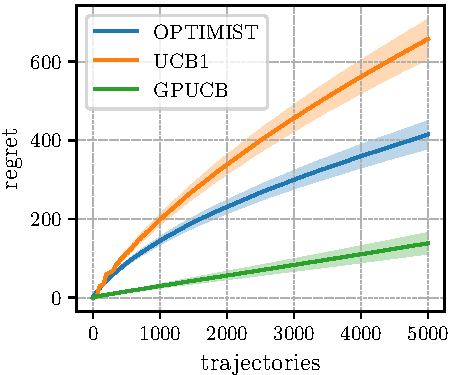
\includegraphics[width=\linewidth]{plots/LQG_mu.pdf}
    \vspace{-0.4cm}
    \caption{Cumulative regret in the LQG experiment, comparing \algoname, UCB1 and GPUCB (30 runs, 95\% c.i.)} 
    \label{fig:lqg} 
  \end{minipage}%%
  \hspace{0.3cm}
  \begin{minipage}[b]{0.24\linewidth}
    \centering
    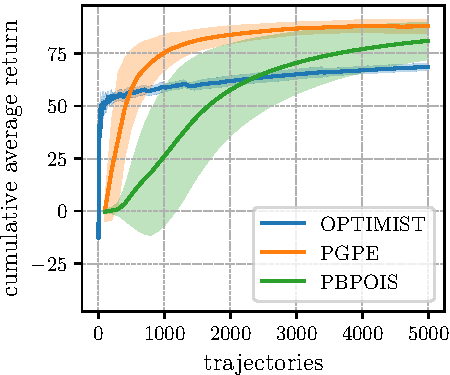
\includegraphics[width=\linewidth]{plots/MC_mu.pdf}
    \vspace{-0.4cm}
    \caption{Cumulative average return for the Mountain Car, comparing \algoname, PGPE and PB-POIS (5 runs, 95\% c.i.)} 
    \label{fig:mc} 
  \end{minipage} %%
  \hspace{0.3cm}
  \begin{minipage}[b]{0.48\linewidth}
    \centering
    \includegraphics[width=0.4\linewidth]{example-image-a}
    \includegraphics[width=0.4\linewidth]{example-image-b}
    \caption{HEATMAPS} 
    \label{fig:mc} 
  \end{minipage} %%
  \vskip -0.2in
\end{figure*}
%
%\begin{figure*}[t]
%\begin{subfigure}
%  \centering
%  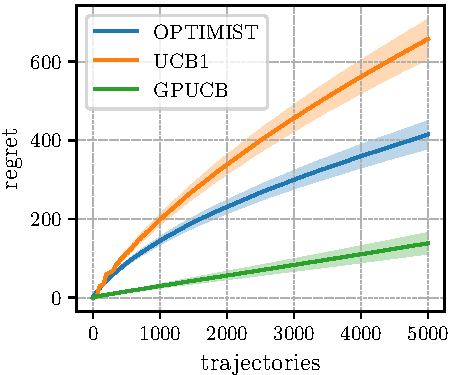
\includegraphics[width=0.24\linewidth]{plots/LQG_mu.pdf}
%  \label{fig:lqg}
%\end{subfigure}
%\begin{subfigure}
%  \centering
%  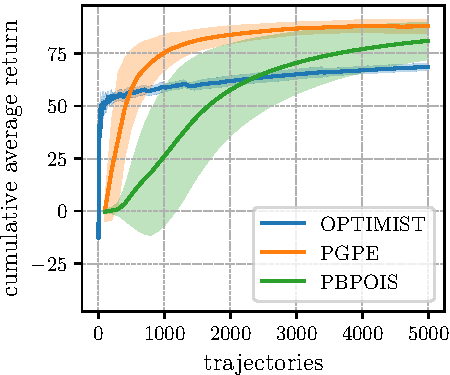
\includegraphics[width=0.24\linewidth]{plots/MC_mu.pdf}
%  \label{fig:mc}
%\end{subfigure}
%\begin{subfigure}
%  \centering
%  \includegraphics[width=0.24\linewidth]{example-image-a}
%  \label{fig:mc1}
%\end{subfigure}
%\begin{subfigure}
%  \centering
%  \includegraphics[width=0.24\linewidth]{example-image-a}
%  \label{fig:mc2}
%\end{subfigure}
%\end{figure*}

\section{Numerical Simulations}\label{sec:exp}
In this section, we present the results of the numerical simulation of \algoname on RL tasks
on both discrete and continuous parameter spaces. We restrict our experiments to the \emph{parameter-based} PS and Gaussian hyperpolicies. This setting is particularly convenient as the \Renyi divergence between Gaussian distributions admits closed form~\cite{gil2013renyi}. On the contrary, in the action-based scenario, 
we would need to compute divergences between trajectory distributions, which is intractable. The usual approach consists in estimating the \Renyi divergence from samples. However, we would lose our theoretical guarantees on the regret. Furthermore, the known estimators for the \Renyi divergence tend empirically to be unstable~\cite{metelli2018policy}. It is worth noting that at each iteration \algoname needs to compute the \Renyi divergence between a candidate hyperpolicy $\nu_{\vxi_t}$ and the mixture of hyperpolicies visited so far $\nu_{\vxi_0}, ..., \nu_{\vxi_{t-1}}$. We prove in Appendix~\ref{app:practical} that this quantity can be upper bounded by the harmonic mean of the divergences between the candidate hyperpolicy $\nu_{\vxi_t}$ and each component of the mixture $\nu_{\vxi_{k}}$ for $k=1,...,t-1$. 

\subsection{Linear Quadratic Gaussian Regulator}
The Linear Quadratic Gaussian Regulator~\citep[LQG,][]{dorato1995linear} is a benchmark problem
for continuous control. We consider the monodimensional case in which the state space restricted to $\mathcal{S}=[-4,4]$, the action space is $\mathcal{A}=[-4,4]$ and the horizon is limited to 20. We employ a Gaussian hyperpolicy $\nu_{\xi} = \mathcal{N}( \xi, \sigma^2)$, where $\xi$ is the mean parameter to be learned and $\sigma=0.15$ fixed. The case in which we learn the standard deviation too is reported in Appendix~\ref{apx:additionalExperiments}.

The goal of this experiment is to compare \algoname
with classical MAB algorithms, especially UCB1~\cite{auer2002finite} and GPUCB~\cite{srinivas2010gaussian} when the parameter space $\Xi$ is discrete. For this purpose we consider
a uniform discretization of the interval $[-1,1]$ made of 100 arms. All algorithms are run with confidence level $\delta=0.2$.
In Figure~\ref{fig:lqg}, we show the cumulative regret averaged over 30 runs of \algoname compared with UCB1 and GPUCB. We can see that our algorithm significantly outperforms UCB1. Indeed, \algoname is
able to exploit the structure of arms, \ie hyperpolicies, by means of the MIS estimation, whereas UCB1 does not make any assumption on arm correlation. On the contrary, GPUCB shows a better performance \wrt to \algoname. We point out that GPUCB requires to specify, at the beginning of learning, the kernel of the Gaussian Process (GP) from which the payoff function is sampled. We employed
the default scikit-learn kernel (RBF) which invalidates all theoretical guarantees, as our payoff is not sampled from a GP.\footnote{Indeed, GPUCB showed a significantly more exploitative behavior \wrt UCB1 and \algoname in the experiment.}

\subsection{Mountain Car}
The second experiment we present aims at showing the learning performance of \algoname  
when the parameters of the hyperpolicy belong to a compact (continuous) space. We consider
the continuous Mountain Car environment.

\section{Conclusion}\label{sec:end}
We have studied the problem of exploration versus exploitation in policy optimization using MAB techniques. We have proposed OPTIMIST, an optimism-based approach for both the action-based and the parameter-based exploration frameworks, and for both discrete and continuous parameter spaces. We have proved sublinear regret bounds for OPTIMIST under assumptions that are easily satisfied in practice. Evaluation on continuous control tasks showed that the proposed algorithms are effectively able to leverage the structure of the PO problem, although performances are not optimal when compared with methods with stronger assumptions or without guarantees, at least on these simple problems.
Future work should focus on finding more efficient (but still effective) ways to perform optimization in the infinite-arm setting, and on applying OPTIMIST also to the action-based framework, which requires additional caveats in computing the exploration bonus.

% Acknowledgements should only appear in the accepted version.
%\section*{Acknowledgements}
%
%\textbf{Do not} include acknowledgements in the initial version of
%the paper submitted for blind review.
%
%If a paper is accepted, the final camera-ready version can (and
%probably should) include acknowledgements. In this case, please
%place such acknowledgements in an unnumbered section at the
%end of the paper. Typically, this will include thanks to reviewers
%who gave useful comments, to colleagues who contributed to the ideas,
%and to funding agencies and corporate sponsors that provided financial
%support.

\bibliography{../biblio}
\bibliographystyle{icml2019}


%%%%%%%%%%%%%%%%%%%%%%%%%%%%%%%%%%%%%%%%%%%%%%%%%%%%%%%%%%%%%%%%%%%%%%%%%%%%%%%
%%%%%%%%%%%%%%%%%%%%%%%%%%%%%%%%%%%%%%%%%%%%%%%%%%%%%%%%%%%%%%%%%%%%%%%%%%%%%%%
% SUPPLEMENTARY MATERIALS
%%%%%%%%%%%%%%%%%%%%%%%%%%%%%%%%%%%%%%%%%%%%%%%%%%%%%%%%%%%%%%%%%%%%%%%%%%%%%%%
%%%%%%%%%%%%%%%%%%%%%%%%%%%%%%%%%%%%%%%%%%%%%%%%%%%%%%%%%%%%%%%%%%%%%%%%%%%%%%%
\clearpage
\onecolumn
\appendix

\section{Upper Bound for the Exponentiated Renyi Divergence between mixtures}\label{app:practical}
\algoname requires at each iteration to compute the exponentiated \Renyi divergence between the currently considered distribution $p_{\vx}$ 
and the mixture $\Phi_t$, \ie $d_{1+\epsilon}(p_{\vx}\|\Phi_t)$. Even for Gaussian distributions, this quantity cannot be obtained in closed form, while
the \Renyi divergence between Gaussians can be computed exactly. In this section, we provide an upper bound for computing the exponentiated \Renyi divergence
between a generic distribution and a mixture.
\begin{restatable}{theorem}{armonic}\label{th:armonic}
	Let $P$ be a probability measure and $\Phi = \sum_{k=1}^K \beta_k Q_k$, with $\beta_k \in [0,1]$ and $\sum_{k=1}^K \beta_k =1$, be a finite mixture of the
	probability measures $\{Q_k\}_{k=1}^K$. Then, for any $\alpha \ge 1$, the exponentiated $\alpha$-\Renyi divergence can be bounded as: 
	\begin{equation*}
	d_{\alpha}(P \| \Phi) \le \frac{1} {\sum_{k=1}^K \frac{ \beta_k}{ d_{\alpha}(P \| Q_k)}}.
	\end{equation*}
\end{restatable}

In Appendix~\ref{app:proof}, we prove a more general result for the case when also $P$ is a mixture.

\section{Proofs}\label{app:proof}

\misevarbound*
%
\begin{proof}
	The proof is similar to Lemma 4.1 of~\cite{metelli2018policy}:
    \begin{align}
    \Var_{z_{ik} \simiid Q_k} [\widehat{\mu}_{\text{BH}}]&  = \Var_{z_{ik} \simiid Q_k} \left[ \frac{1}{N} \sum_{k=1}^K \sum_{i=1}^{N_k}  f(z_{ki})\frac{p(z_{ki})}{\sum_{j=1}^n \frac{N_j}{N} q_j(z_{ki})} \right] \notag \\
    & = \frac{1}{N^2} \sum_{k=1}^K \sum_{i=1}^{N_k} \Var_{z_{ik} \sim Q_k} \left[   f(z_{ki}) \frac{p(z_{ki})}{\sum_{j=1}^n \frac{N_j}{N} q_j(z_{ki})} \right] \label{p:misevarboundline2} \\
    & \le \frac{1}{N^2} \sum_{k=1}^K \sum_{i=1}^{N_k} \Exp_{z_{ik} \sim Q_k} \left[   \left( f(z_{ki})   \frac{p(z_{ki})}{\sum_{j=1}^n \frac{N_j}{N} q_j(z_{ki})} \right)^2 \right] \notag\\
    & \le \|f\|_{\infty} \frac{1}{N^2} \sum_{k=1}^K \sum_{i=1}^{N_k} \Exp_{z_{ik} \sim Q_k} \left[   \left( \frac{p(z_{ki})}{\sum_{j=1}^n \frac{N_j}{N} q_j(z_{ki})} \right)^2 \right]  \notag\\
    & = \|f\|_{\infty}^2 \frac{1}{N} \Exp_{z \sim \Phi} \left[ \left(\frac{p(z)}{\sum_{j=1}^n \frac{N_j}{N} q_j(z)} \right)^2 \right] \label{p:misevarboundline5}\\
    &= \|f\|_{\infty}^2 \frac{d_{2}(P\|\Phi)}{N},  \notag
    \end{align}
    where~\eqref{p:misevarboundline2} follows from the independence of the $z_{ik}$ and~\eqref{p:misevarboundline5} is obtained by the definition of $\Phi$ and observing that for an arbitrary function $g$:
    \begin{equation}
    \label{eq:expectationdecomposition}
    	\frac{1}{N} \sum_{k=1}^K \sum_{i=1}^{N_k} \Exp_{z_{ik} \sim Q_k}[g(z_{ik})] =  \sum_{k=1}^K \frac{N_k}{N} \Exp_{z_{1k} \sim Q_k}[g(z_{1k})] = \Exp_{z \sim \Phi}[g(z)].
    \end{equation}
\end{proof}


\truncatedbias*
\begin{proof}
Let us start with the bias term. The first inequality $0 \le \mu - \Exp_{z_{ik} \simiid Q_k} [\widecheck{\mu}_{\text{BH}}]$ derives from the fact that $\widehat{\mu}_{\text{BH}} \ge \widecheck{\mu}_{\text{BH}}$, being $f(z) \ge 0$ for all $z$ and observing that $\widehat{\mu}$ is unbiased, \ie $\Exp_{z_{ik} \simiid Q_k}[\widehat{\mu}_{\text{BH}}]=\mu$. For the second inequality, let us consider the following derivation:
    \begin{align}
    \mu - \Exp_{x_i \sim q_i} [\widecheck{\mu}]&  = \Exp_{z_{ik} \simiid Q_k}[\widehat{\mu}_{\text{BH}}] - \Exp_{z_{ik} \simiid Q_k} [\widecheck{\mu}_{\text{BH}}] \notag \\
    & =  \frac{1}{N} \sum_{k=1}^K\sum_{i=1}^{N_k} \Exp_{z_{ik} \sim Q_k} \left[  f(z_{ik}) \left( \frac{p(z_{ik})}{\sum_{j=1}^K \frac{N_j}{N} q_j(z_{ik})} - \min \left\{ M,  \frac{p(z_{ik})}{\sum_{j=1}^K \frac{N_j}{N} q_j(z_{ik})} \right\} \right) \right]\\    
%    & =   \sum_{k=1}^K \frac{N_k}{N} \Exp_{z_{1k} \sim Q_k} \left[  f(z_{1k}) \left( \frac{p(z_{1k})}{\sum_{j=1}^K \frac{N_j}{N} q_j(z_{1k})} - \min \left\{ M,  \frac{p(z_{1k})}{\sum_{j=1}^K \frac{N_j}{N} q_j(z_{1k})} \right\} \right) \right] \\
%     & = \Exp_{z \sim \Phi} \left[  f(z) \left( \frac{p(z)}{\sum_{j=1}^K \frac{N_j}{N} q_j(z)} - \min \left\{ M,  \frac{p(z)}{\sum_{j=1}^K \frac{N_j}{N} q_j(z)} \right\} \right) \right]\\
    & =  \Exp_{z \sim \Phi} \left[  f(z) \left(  \frac{p(z)}{\sum_{j=1}^K \frac{N_j}{N} q_j(z)} - M  \right) \mathds{1}_{\left\{ \frac{p(z)}{\sum_{j=1}^K \frac{N_j}{N} q_j(z)} \ge M \right\} } \right] \label{p:truncatedbias1}\\
    & \le \Exp_{z \sim \Phi} \left[  f(z) \left(  \frac{p(z)}{\sum_{j=1}^K \frac{N_j}{N} q_j(z)} \right) \mathds{1}_{\left\{ \frac{p(z)}{\sum_{j=1}^K \frac{N_j}{N} q_j(z)} \ge M \right\} } \right] \label{p:truncatedbias2}\\
    & \le \|f\|_{\infty} \Exp_{z \sim \Phi} \left[  \left(  \frac{p(z)}{\sum_{j=1}^K \frac{N_j}{N} q_j(z)} \right) \mathds{1}_{\left\{ \frac{p(z)}{\sum_{j=1}^K \frac{N_j}{N} q_j(z)} \ge M \right\} } \right] \notag\\
    & \le \|f\|_{\infty} \Exp_{z \sim \Phi} \left[  \left(  \frac{p(z)}{\sum_{j=1}^K \frac{N_j}{N} q_j(z)} \right)^{1+\epsilon} \left(  \frac{p(z)}{\sum_{j=1}^K \frac{N_j}{N} q_j(z)} \right)^{-\epsilon} \mathds{1}_{\left\{ \frac{p(z)}{\sum_{j=1}^K \frac{N_j}{N} q_j(z)} \ge M \right\} } \right] \notag\\
    & \le \|f\|_{\infty} \Exp_{z \sim \Phi} \left[  \left(  \frac{p(z)}{\sum_{j=1}^K \frac{N_j}{N} q_j(z)} \right)^{1+\epsilon} \right] M^{-\epsilon} \label{p:truncatedbias3}\\
        & = \|f\|_{\infty} d_{1+\epsilon}(P \| \Phi)^{\epsilon}  M^{-\epsilon},\notag
    \end{align}
    where~\eqref{p:truncatedbias1} is an application of equation~\eqref{eq:expectationdecomposition}, \eqref{p:truncatedbias2} derives from recalling that $M\ge 0$ and \eqref{p:truncatedbias3} is obtained by observing that $ x^{-\epsilon} \mathds{1}_{\left\{ x \ge M \right\} }$ is either $0$ and thus the bound holds or at most $M^{-\epsilon}$.
    For the variance the argument is similar:
    \begin{align}
    \Var_{z_{ik} \simiid Q_k} [\widecheck{\mu}_{\text{BH}}]&  = \Var_{z_{ik} \simiid Q_k} \left[ \frac{1}{N} \sum_{k=1}^K \sum_{i=1}^{N_k}  f(z_{ki}) \min \left\{ M, \frac{p(z_{ki})}{\sum_{j=1}^n \frac{N_j}{N} q_j(z_{ki})} \right\} \right] \notag\\
    & = \frac{1}{N^2} \sum_{k=1}^K \sum_{i=1}^{N_k} \Var_{z_{ik} \sim Q_k} \left[   f(z_{ki}) \min \left\{ M, \frac{p(z_{ki})}{\sum_{j=1}^n \frac{N_j}{N} q_j(z_{ki})} \right\} \right] \notag\\
    & \le \frac{1}{N^2} \sum_{k=1}^K \sum_{i=1}^{N_k} \Exp_{z_{ik} \sim Q_k} \left[   \left( f(z_{ki})  \min \left\{ M, \frac{p(z_{ki})}{\sum_{j=1}^n \frac{N_j}{N} q_j(z_{ki})} \right\} \right)^2 \right]\notag\\
    & \le \|f\|_{\infty} \frac{1}{N^2} \sum_{k=1}^K \sum_{i=1}^{N_k} \Exp_{z_{ik} \sim Q_k} \left[   \left( \min \left\{ M, \frac{p(z_{ki})}{\sum_{j=1}^n \frac{N_j}{N} q_j(z_{ki})} \right\} \right)^2 \right]\notag\\
    & = \|f\|_{\infty}^2 \frac{1}{N} \Exp_{z \sim \Phi} \left[ \min \left\{ M, \frac{p(z)}{\sum_{j=1}^n \frac{N_j}{N} q_j(z)} \right\}^2 \right] \label{p:truncatedbias4}\\
    & = \|f\|_{\infty}^2 \frac{1}{N} \Exp_{z \sim \Phi} \left[ \min \left\{ M, \frac{p(z)}{\sum_{j=1}^n \frac{N_j}{N} q_j(z)} \right\}^{1+\epsilon} \min \left\{ M, \frac{p(z)}{\sum_{j=1}^n \frac{N_j}{N} q_j(z)} \right\}^{1-\epsilon}  \right]\notag\\
    & \le \|f\|_{\infty}^2 \frac{1}{N} \Exp_{z \sim \Phi} \left[ \left( \frac{p(z)}{\sum_{j=1}^n \frac{N_j}{N} q_j(z)} \right)^{1+\epsilon}  \right] M^{1-\epsilon} \label{p:truncatedbias5}\\
    &= \|f\|_{\infty}^2 M^{1-\epsilon} \frac{d_{1+\epsilon}(P\|\Phi)^{\epsilon}}{N} ,\notag\\
    \end{align}
    where~\eqref{p:truncatedbias4}  is again an application of equation~\eqref{eq:expectationdecomposition} and~\ref{p:truncatedbias5} derives from observing that $\min\{x,y\} \le x$ and also $\min\{x,y\} \le y$.
\end{proof}

\thrucatedconcentration*

\begin{proof}
Let us start with the first inequality. Observing that all samples $z_{ik}$ are independent and that $\widecheck{\mu}_{\text{BH}} \le M \|f\|_{\infty}$, we can state using Bernstein inequality~\cite{boucheron2013concentration} that with probability at least $1-\delta$ we have:
    \begin{align}
         \widecheck{\mu}_{\text{BH}} & \le \Exp_{z_{ik} \sim Q_k} [\widecheck{\mu}_{\text{BH}}] + \sqrt{2 \Var_{z_{ik} \simiid Q_k}[\widecheck{\mu}_{\text{BH}}] \log \frac{1}{\delta}} +\|f\|_{\infty}  \frac{M  \log \frac{1}{\delta}}{3N} \notag \\
         & \le \mu + \|f\|_{\infty} \sqrt{\frac{2 M^{1-\epsilon} d_{1+\epsilon}\left( P \| \Phi \right)^{\epsilon} \log  \frac{1}{\delta} }{N}} +\|f\|_{\infty} \frac{M \log \frac{1}{\delta}}{3N} \label{p:thrucatedconcentration1}\\
       & = \mu + \|f\|_{\infty}\left(\sqrt{2} + \frac{1}{3} \right)  \left(\frac{d_{1+\epsilon}\left( P \| \Phi  \right) \log  \frac{1}{\delta}  }{N} \right)^{\frac{\epsilon}{1+\epsilon}} \label{p:thrucatedconcentration2},
    \end{align}
    where~\eqref{p:thrucatedconcentration1} is obtained by substituting the variance with its bound~\eqref{eq:variancetruncated} and~\eqref{p:thrucatedconcentration2} is from the choice of $M$.
    For the second inequality we just need to consider additionally the bias.
    \begin{align}
         \widecheck{\mu}_{\text{BH}} & \ge  \Exp_{z_{ik} \sim Q_k} [\widecheck{\mu}_{\text{BH}}] - \sqrt{2 \Var_{z_{ik} \simiid Q_k}[\widecheck{\mu}_{\text{BH}}] \log \frac{1}{\delta}} -\|f\|_{\infty}  \frac{M  \log \frac{1}{\delta}}{3N} \notag\\
         & = \mu - \left(\mu - \Exp_{z_{ik} \sim Q_k} [\widecheck{\mu}_{\text{BH}}] \right) -\sqrt{2 \Var_{z_{ik} \simiid Q_k}[\widecheck{\mu}_{\text{BH}}] \log \frac{1}{\delta}} -\|f\|_{\infty}  \frac{M  \log \frac{1}{\delta}}{3N}  \notag\\
          & \ge \mu - \|f\|_{\infty} M^{-\epsilon} d_{1+\epsilon}\left( P \| \Phi \right)^{\epsilon} - \|f\|_{\infty}\left(\sqrt{2} + \frac{1}{3} \right)  \left(\frac{d_{1+\epsilon}\left( P \| \Phi  \right) \log  \frac{1}{\delta}  }{N} \right)^{\frac{\epsilon}{1+\epsilon}} \label{p:thrucatedconcentration3}\\
          & = \mu - \|f\|_{\infty} \left(\sqrt{2} + \frac{4}{3} \right) \left(\frac{d_{1+\epsilon}\left( P \| \Phi  \right) \log  \frac{1}{\delta}  }{N} \right)^{\frac{\epsilon}{1+\epsilon}}, \notag\\
    \end{align}
    where~\eqref{p:thrucatedconcentration3} comes from substituting the bias with its bound~\eqref{eq:biastruncated}.
\end{proof}

%Finite arm set
\regretdiscrete*
%
\begin{proof}
	Fix an $\epsilon>0$.
	To ease the notation, let $c^{-}\coloneqq \norm[\infty]{f}\left(\sqrt{2}+\frac{1}{3}\right)$, $c^{+}\coloneqq \norm[\infty]{f}\left(\sqrt{2}+\frac{4}{3}\right)$, and $\beta_t(\vx) \coloneqq \left(\frac{d_{1+\epsilon}(p_{\vx}\|\Phi_t)\log\frac{1}{\delta_t}}{t}\right)^{\frac{\epsilon}{1+\epsilon}}$.
	We start by showing that, with probability at least $1-\delta$:
	\begin{align}\label{aux:1}
		&-c^{+}\beta_t({\vx})\leq \wc{\mu_t}(\vx) - \mu(\vx) \leq c^{-}\beta_t(\vx) & \text{for all $\vx\in\Xspace$ and $t=1,\dots,T$}.
	\end{align}
	Indeed:
	\begin{align}
		\Prob\left(\bigcap_{k=1}^{K}\bigcap_{t=1}^T\left[\wc{\mu_t}(\vx_k) - \mu(\vx_k) \leq c^{-}\beta_t(\vx_k)\right]\right) &=1-\Prob\left(\bigcup_{k=1}^{K}\bigcup_{t=1}^T\left[\wc{\mu_t}(\vx_k) - \mu(\vx_k) > c^{-}\beta_t(\vx_k)\right]\right)\nonumber\\
		&\geq 1-K\sum_{t=1}^{T}\Prob\left(\wc{\mu_t}(\vx_1) - \mu(\vx_1) > c^{-}\beta_t(\vx_1)\right) \label{pp:1}\\
		& \geq 1 - K\sum_{t=1}^{T}\delta_t\label{pp:2}\\
		& \geq 1 - \frac{\delta}{2},\label{pp:3}
	\end{align}
	where (\ref{pp:1}) is from a double union bound (over time and over the finite elements of $\Xspace$), (\ref{pp:2}) is from Theorem \ref{lem:thrucatedconcentration}, and (\ref{pp:3}) is by hypothesis on $\delta_t$ and $\sum_{t=1}^{T}\frac{1}{t^2}\leq\sum_{t=1}^{\infty}\frac{1}{t^2} = \frac{\pi^2}{6}$. Similarly:
	\begin{align*}
		\Prob\left(\bigcap_{k=1}^{K}\bigcap_{t=1}^T\left[\wc{\mu_t}(\vx_k) - \mu(\vx_k) \geq -c^{+}\beta_t(\vx_k)\right]\right) &=1-\Prob\left(\bigcup_{k=1}^{K}\bigcup_{t=1}^T\left[\wc{\mu_t}(\vx_k) - \mu(\vx_k) < -c^{+}\beta_t(\vx_k)\right]\right)\nonumber\\
		&\geq 1-K\sum_{t=1}^{T}\Prob\left(\wc{\mu_t}(\vx_1) - \mu(\vx_1) < -c^{+}\beta_t(\vx_1)\right)\\
		&\geq 1 - K\sum_{t=1}^{T}\delta_t\\
		 &\geq 1 - \frac{\delta}{2}.
	\end{align*}
	Hence, by union bound over the two inequalities, (\ref{aux:1}) holds with probability at least $1-\delta$.
	This allows to lower bound the instantaneous regret with the same probability:
	\begin{align}
		\Delta_t &= \mu(\vx^*) - \mu(\vx) \leq 
		\wc{\mu_t}(\vx^*) + c^{+}\beta_t(\vx^*) - \mu(\vx_t) \label{pp:4}\\
		&\leq \wc{\mu_t}(\vx_t) + c^{+}\beta_t(\vx_t) - \mu(\vx_t) \label{pp:5}\\
		&\leq (c^{-} + c^{+})\beta(\vx_t) & \text{for all $t=1,\dots,T$}\label{aux:2}, 
	\end{align}
	where (\ref{pp:4}) and (\ref{aux:2}) are from (\ref{aux:1}), while (\ref{pp:5}) is by hypothesis, as $\vx_t=\arg\max_{\vx\in\Xspace}(\wc{\mu_t}(\vx) + c^{+}\beta_t(\vx))$.
	Note that the union bound over the elements of $\Xspace$ in (\ref{aux:1}) was necessary for (\ref{pp:4}) as the optimal arm $\vx^*$ may not be unique.
	Finally, with probability at least $1-\delta$:
	\begin{align}
		\Reg(T) &= \sum_{t=0}^{T}\Delta_t \nonumber\\
		&= \Delta_0  + \sum_{t=1}^{T}\Delta_t \nonumber\\
		&\leq \Delta_0  + (c^{+}+c^{-})\sum_{t=1}^{T}\beta_t(\vx_t) \label{pp:6}\\
		&\leq \Delta_0  + (c^{+}+c^{-})v_{\epsilon}^{\frac{\epsilon}{1+\epsilon}}\sum_{t=1}^{T}\left(\frac{\log\frac{1}{\delta_t}}{t}\right)^{\frac{\epsilon}{1+\epsilon}} \label{pp:7}\\
		&=\Delta_0  + (c^{+}+c^{-})v_{\epsilon}^{\frac{\epsilon}{1+\epsilon}}\sum_{t=1}^{T}\left(\frac{2\log t + \log\frac{\pi^2K}{3\delta}}{t}\right)^{\frac{\epsilon}{1+\epsilon}} \label{pp:8}\\
		&\leq \Delta_0  + (c^{+}+c^{-})\left[v_{\epsilon}\left(2\log T + \log\frac{\pi^2K}{3\delta}\right)\right]^{\frac{\epsilon}{1+\epsilon}}\sum_{t=1}^{T}t^{-\frac{\epsilon}{1+\epsilon}} \nonumber\\
		&\leq \Delta_0  + (c^{+}+c^{-})\left[v_{\epsilon}\left(2\log T + \log\frac{\pi^2K}{3\delta}\right)\right]^{\frac{\epsilon}{1+\epsilon}}(1+\epsilon)T^{\frac{1}{1+\epsilon}} \label{pp:9},
	\end{align}
	where (\ref{pp:6}) is from (\ref{aux:2}) and holds with probability no less than $1-\delta$, (\ref{pp:7}) is from Assumption \ref{ass:boundrenyi}, (\ref{pp:8}) is by definition of $\delta_t$, and (\ref{pp:9}) is from: 
	\begin{align}\label{aux:3}
		&\sum_{t=1}^{T}t^{-\alpha} \leq \int_{1}^{T+1}t^{-\alpha}\de t
		= \frac{1}{1-\alpha}\left((T+1)^{1-\alpha} - 1\right) \leq \frac{T^{1-\alpha}}{1-\alpha} &\text{for all $0<\alpha<1$},
	\end{align}
	with $\alpha=\frac{\epsilon}{1+\epsilon}$.
	The proof is completed by renaming $C\gets (1+\epsilon)(c^{+}+c^{-}) = (1+\epsilon)(2\sqrt{2} + \frac{5}{3})\norm[\infty]{f}$.
\end{proof}

%Compact case
\lipschitzpol*
\begin{proof}
	We consider the infinite-horizon case ($H=\infty,\gamma<1$), as the finite-horizon case is \wlg under mild assumptions.
	To show Lipschitz continuity in the action-based paradigm, it is enough to bound $\norm[\infty]{\nabla_{\vtheta}J}$ under (\ref{eq:lp1}). From the Policy Gradient Theorem~\cite{sutton2000policy}:
	\begin{align}\label{aux:4}
		\nabla_{\vtheta}J(\vtheta) = \frac{1}{1-\gamma}\Exp_{\substack{s\sim \rho_{\vtheta}
		\\a\sim\pi_{\vtheta}}}\left[\nabla_{\vtheta}\log\pi_{\vtheta}(a|s)Q_{\vtheta}(s,a)\right],
	\end{align}
	where $\rho_{\vtheta}$ is the discounted state-occupancy measure under policy $\pi_{\vtheta}$ and $Q_{\vtheta}$ is the action-value function~\cite{sutton2000policy}, modeling the reward that can be obtained starting from state $s$, taking action $a$ and following $\pi_{\vtheta}$ thereafter.
	From (\ref{aux:4}), for every $\vtheta\in\Theta$:
	\begin{align}
		|\nabla_{\vtheta}J(\vtheta)| 
		&\leq \frac{\Rmax}{(1-\gamma)^2}\Exp_{\substack{s\sim \rho_{\vtheta}\\a\sim\pi_{\vtheta}}}\left[|\nabla_{\vtheta}\log\pi_{\vtheta}(s,a)|\right] \label{pp:10}\\
		&\leq \frac{\Rmax}{(1-\gamma)^2}\sup_{s\in\Sspace}\Exp_{a\sim\pi_{\vtheta}}\left[|\nabla_{\vtheta}\log\pi_{\vtheta}(s,a)|\right] \nonumber\\
		& = \frac{\vu_1\Rmax}{(1-\gamma)^2}, \label{pp:11}
	\end{align}
	where the inequalities are component-wise, (\ref{pp:10}) is from the trivial fact $\norm[\infty]{Q_{\vtheta}}\leq\frac{\Rmax}{(1-\gamma)}$, and (\ref{pp:11}) is from assumption (\ref{eq:lp1}). It follows that $L=\frac{\norm[\infty]{\vu_1}\Rmax}{(1-\gamma)^2}$ is a valid Lipschitz constant under the $l_1$ norm.
	The commonly used Gaussian policy:
	\begin{align}\label{eq:gauss}
		\pi_{\vtheta}(a|s) = \mathcal{N}(\vtheta^T\vphi(s),\sigma^2)  = \frac{1}{\sqrt{2\pi}\sigma}\exp\left\{-\frac{1}{2}\left(\frac{a-\vtheta^T\vphi(s)}{\sigma}\right)^2\right\},
	\end{align}
	where $\phi(s)$ is a vector of component-wise bounded state features, \ie $\sup_{s\in\Sspace}|\vphi(s)|\leq \vphi_{\max}$, satisfies assumption (\ref{eq:lp1}):
	\begin{align}
		\Exp_{a\sim\pi_{\vtheta}}\left[\left|\nabla_{\vtheta}\log\pi_{\vtheta}(a|s)\right|\right] 
		&=\Exp_{a\sim\pi_{\vtheta}}\left[\frac{|\vphi(s)(a-\vtheta^T\vphi(s))|}{\sigma^2}\right] \nonumber\\
		&\leq \frac{|\vphi(s)|}{\sigma}\Exp_{a\sim\pi_{\vtheta}}\left[\left|\frac{a-\vtheta^T\vphi(s)}{\sigma}\right|\right] \nonumber\\
		&\leq \frac{|\vphi(s)|}{\sqrt{2\pi}\sigma}\int_{\Reals} e^{-x^2}|x|\de x \label{pp:14}\\
		& \leq  \frac{2\vphi_{\max}}{\sqrt{2\pi}\sigma}\coloneqq \vu_1, \label{aux:5}
	\end{align}
	where inequalities are component-wise and (\ref{pp:14}) is by the substitution $x\gets \frac{a-\vtheta^T\vphi(s)}{\sigma}$. Even when $\sigma$ must be learned, proper parametrization (\eg $\sigma\propto\exp\{\vtheta\}$), together with the compactness of $\Theta$, allows to satisfy assumption (\ref{eq:lp1}).
	
	To show Lipschitz continuity for the parameter-based paradigm, it is enough to bound $\norm[\infty]{\nabla_{\vxi}\Exp_{\vtheta\sim\rho_{\vxi}}[J(\vtheta)]}$ under (\ref{eq:lp2}). For every $\vxi\in\Xi$:
	\begin{align}
		\left|\nabla_{\vxi}\Exp_{\vtheta\sim\rho_{\vxi}}[J(\vtheta)]\right| &=
		\left|\Exp_{\vtheta\sim\rho_{\vxi}}[\nabla_{\vxi}\log\rho_{\vxi}(\vtheta)J(\vtheta)]\right| \nonumber\\
		&\leq \frac{\Rmax}{(1-\gamma)}\Exp_{\vtheta\sim\rho_{\vxi}}\left[\left|\nabla_{\vxi}\log\rho_{\vxi}(\vtheta)\right|\right] \label{pp:12} \\
		&\leq \frac{\vu_2\Rmax}{(1-\gamma)} \label{pp:13},
	\end{align}
	where the inequalities are component-wise, (\ref{pp:12}) is from the trivial fact $J(\vtheta)\leq\frac{\Rmax}{1-\gamma}$, and (\ref{pp:13}) is from assumption (\ref{eq:lp2}).
	It follows that $L=\frac{\norm[\infty]{\vu_2\Rmax}}{(1-\gamma)}$ is a valid Lipschitz constant under the $l_1$ norm.
	 A Gaussian hyperpolicy $\rho_{\vxi}(\vtheta) = \mathcal{N}(\vxi,\mathrm{diag}(\boldsymbol{\sigma}))$ satisfies assumption (\ref{eq:lp2}) with $\vu_2 = \frac{2}{\sqrt{2\pi}\boldsymbol{\sigma}}$. The proof of this fact is analogous to that of (\ref{aux:5}). Even when $\boldsymbol{\sigma}$ must be learned, proper parametrization (\eg $\boldsymbol{\sigma}\propto\exp\{\vxi\}$), together with the compactness of $\Xi$, allows to satisfy assumption (\ref{eq:lp2}).
\end{proof}

\regretcompact*
\begin{proof}
	Fix an $\epsilon>0$. Let $c^{-}$, $c^{+}$ and $\beta_t(\vx)$ be defined as in the proof of Theorem \ref{th:regretdiscrete}.
	The finite cardinality of $\Xspace$ allowed to perform a union bound over the arms that was crucial for the proof of Theorem \ref{th:regretdiscrete}. We cannot do the same here as $\Xspace$ has infinite cardinality. To overcome this problem, we follow the line of reasoning proposed by~\citet{srinivas2010gaussian}. First, we can say something about the arms that are actually selected by the algorithm, which are finite. From Theorem \ref{lem:thrucatedconcentration}, by a union bound over $t=1,\dots,T$, we have that, with probability at least $1-\sum_{t=1}^T\delta_t$:
	\begin{align}\label{aux:6}
		&\wc{\mu_t}(\vx_t) - \mu(\vx_t) \leq c^{-}\beta_t(\vx_t) &\text{for all $t=1,\dots,T$}.
	\end{align}
	
	We also need a specular inequality for the optimal arm. Unfortunately, we cannot assume there exists a unique optimal arm $\vx^*$.\footnote{Instead, $\mu(\vx^*$) is always unique.} Even worse, a dense set of optimal arms may exist. To overcome this problem, we introduce, \textit{only for the purposes of the proof}, a discretization of the arm space. Let $\wt{\Xspace}_t$ be a $d$-dimensional regular grid of $\tau_t^d$ vertexes, where $(\tau_t\in\Naturals_{+})_{t=1}^T$ is a discretization schedule. Let $[\vx]_t$ be the closest vertex to $\vx$ in $\wt{\Xspace}_t$. From Assumption \ref{ass:lipschitz}:
	\begin{align}\label{aux:7}
		&|\mu(\vx) - \mu([\vx]_t)| \leq L\norm[1]{\vx - [\vx]_t} \leq \frac{LDd}{\tau_t},
	\end{align}
	as each voxel of the grid has side $\frac{2D}{\tau_t}$ and no point can be further from a vertex than $d$ half-sides according to the $l_1$ norm. Now fix a $t\geq1$ and an optimal arm $\vx^*$. With probability at least $1-\delta_t$:
	\begin{align}
		\mu(\vx^*) - \wc{\mu}_t([\vx^*]_t) 
		&= \mu(\vx^*) - \mu([\vx^*]_t) + \mu([\vx^*]_t) - \wc{\mu}_t([\vx^*]_t)  \nonumber\\
		&\leq \mu([\vx^*]_t) - \wc{\mu}_t([\vx^*]_t) + |\mu(\vx^*) - \mu([\vx^*]_t)| \nonumber\\
		&\leq c^{+}\beta_t([\vx^*]_t) + \frac{LDd}{\tau_t}, \label{aux:8}
	\end{align}
	where the inequality (\ref{aux:8}) is from Theorem \ref{lem:thrucatedconcentration} and (\ref{aux:7}). Since any voxel may contain an optimal arm, we must perform a union bound over the $\lceil\tau\rceil^d$ vertexes of $\wt{\Xspace}_t$, and a subsequent one over $t,\dots,T$. Hence, with probability at least $1-\sum_{t=1}^{T}\tau_t^d\delta_t$:
	\begin{align}\label{aux:9}
		&\mu(\vx^*) - \wc{\mu}_t([\vx^*]_t) \leq c^{+}\beta_t([\vx^*]_t) + \frac{LDd}{\tau_t} &\text{for $t=1,\dots,T$ and every $\vx^*\in\arg\max_{\vx\in\Xspace}\mu(\vx)$}.
	\end{align}
	
	We can now proceed to bound the instantaneous regret. With probability at least $1-\sum_{t=1}^T\delta_t(1+\tau_t^d)$:
	\begin{align}
	\Delta_t = \mu(\vx^*) - \mu(\vx_t) &\leq 
	\wc{\mu_t}([\vx^*]_t) + c^{+}\beta_t([\vx^*]_t) + \frac{LDd}{\tau_t} - \mu(\vx_t) \label{pp:15}\\
	&\leq \wc{\mu_t}(\vx_t) + c^{+}\beta_t(\vx_t) + \frac{LDd}{\tau_t} - \mu(\vx_t) \label{pp:16}\\
		&\leq (c^{+}+c^{-})\beta_t(\vx_t) + \frac{LDd}{\tau_t}, \label{aux:10}
	\end{align}
	where (\ref{pp:15}) is from (\ref{aux:9}) and holds with probability at least $1-\sum_{t=1}^{T}\tau_t^d\delta_t$, (\ref{pp:16}) is by hypothesis, as $\vx_t=\arg\max_{\vx\in\Xspace}(\wc{\mu_t}(\vx) + c^{+}\beta_t(\vx))$, and (\ref{aux:10}) is from (\ref{aux:7}) and holds with probability at least $1-\sum_{t=1}^{T}\delta_t$. Hence, (\ref{aux:10}) holds with probability no less than $1-\sum_{t=1}^{T}\tau_t^d\delta_t - \sum_{t=1}^{T}\delta_t = 1 - \sum_{t=1}^T\delta_t(1+\tau_t^d)$. Let us pick as a discretization schedule $\tau_t = dt^2$. This has no impact whatsoever on the algorithm, as the discretization is only hypothetical. With this $\tau_t$ and the confidence schedule proposed in the statement of the theorem, it is easy to verify that (\ref{aux:10}) holds with probability at least $1-\delta$.
	
	Finally, we can bound the regret. With probability at least $1-\delta$:
	\begin{align}
		\Reg(T) &\leq \Delta_0 + \sum_{t=1}^{T}\Delta_t \nonumber\\
		&\leq \Delta_0 + (c^{+}+c^{-})\sum_{t=1}^{T}\beta_t(\vx_t) + LDd\sum_{t=1}^{T}\frac{1}{\tau_t} \label{pp:17}\\
		&\leq (c^{+}+c^{-})\sum_{t=1}^{T}\beta_t(x_t) + \frac{\pi^2LD}{6} \label{pp:18}\\
		&\leq \Delta_0 + (c^{+}+c^{-})v_{\epsilon}^{\frac{\epsilon}{1+\epsilon}}\sum_{t=1}^{T}\left(\frac{\log\frac{1}{\delta_t}}{t}\right)^{\frac{\epsilon}{1+\epsilon}} + \frac{\pi^2LD}{6} \label{pp:19}\\
		&\leq \Delta_0 + (c^{+}+c^{-})v_{\epsilon}^{\frac{\epsilon}{1+\epsilon}}\sum_{t=1}^{T}\left(\frac{
			\log (1+d^dt^{2d}) + 2\log t + \log\frac{\pi^2}{6\delta}
		}{t}\right)^{\frac{\epsilon}{1+\epsilon}} + \frac{\pi^2LD}{6} \label{pp:20}\\
		&\leq \Delta_0 + (c^{+}+c^{-})v_{\epsilon}^{\frac{\epsilon}{1+\epsilon}}\sum_{t=1}^{T}\left(\frac{
		\log (2d^dt^{2d}) + 2\log t + \log\frac{\pi^2}{6\delta}
		}{t}\right)^{\frac{\epsilon}{1+\epsilon}} + \frac{\pi^2LD}{6} \label{pp:21}\\
		&= \Delta_0 + (c^{+}+c^{-})v_{\epsilon}^{\frac{\epsilon}{1+\epsilon}}\sum_{t=1}^{T}\left(\frac{
		2(d+1)\log t + d\log d + \log\frac{\pi^2}{3\delta}
		}{t}\right)^{\frac{\epsilon}{1+\epsilon}} + \frac{\pi^2LD}{6} \nonumber\\
		&\leq \Delta_0 + (c^{+}+c^{-})\left[v_{\epsilon}\left(
			2(d+1)\log T + d\log d + \log\frac{\pi^2}{3\delta}
		\right)\right]^{\frac{\epsilon}{1+\epsilon}}\sum_{t=1}^{T}
		t^{-\frac{\epsilon}{1+\epsilon}} + \frac{\pi^2LD}{6} 	\nonumber\\
		&\leq \Delta_0 + (c^{+}+c^{-})\left[v_{\epsilon}\left(
		2(d+1)\log T + d\log d + \log\frac{\pi^2}{3\delta}
		\right)\right]^{\frac{\epsilon}{1+\epsilon}}(1+\epsilon)T^{\frac{1}{1+\epsilon}}+ \frac{\pi^2LD}{6}, 	\label{pp:22}
	\end{align}
	where (\ref{pp:17}) is from (\ref{aux:10}) and holds with probability at least $1-\delta$, (\ref{pp:18}) is from the choice of $\tau_t$ and $\sum_{t=1}^{T}t^{-2}\leq\sum_{t=1}^{\infty}t^{-2} = \frac{\pi^2}{6}$, (\ref{pp:19}) is from Assumption \ref{ass:boundrenyi}, (\ref{pp:20}) is from the choice of $\delta_t$, (\ref{pp:21}) is from $\log(1+x)\leq\log(2x)$, which holds for every $x\geq 1$, and (\ref{pp:22}) is from  (\ref{aux:3}) with $\alpha=\frac{\epsilon}{1+\epsilon}$. 
	The proof is completed by renaming $C\gets (1+\epsilon)(c^{+}+c^{-}) = (1+\epsilon)(2\sqrt{2} + \frac{5}{3})\norm[\infty]{f}$.
\end{proof}

\regretdiscretized*
\begin{proof}
	The proof follows the one of Theorem \ref{th:regretcompact} up to (\ref{aux:9}), except from the fact that the discretization is actually performed by the algorithm. That is, with probability at least $1-\sum_{t=1}^{T}\delta_t(1+\tau_t^d)$:
	\begin{align}
		&\wc{\mu}_t(\vx_t) - \mu(\vx_t) \leq c^{-}\beta_t(\vx_t) &\text{and}\nonumber\\
		&\mu(\vx^*) - \wc{\mu}_t([\vx^*]_t) \leq c^{+}\beta_t([\vx^*]_t) + \frac{LDd}{\tau_t}
		&\text{for $t=1,\dots,T$ and every $\vx^*\in\arg\max_{\vx\in\Xspace}\mu(\vx)$.}\label{aux:11}
	\end{align}
	This is enough to bound the instantaneous regret. With probability at least $1-\sum_{t=1}^{T}\delta_t(1+\tau_t^d)$:
	\begin{align}
		\Delta_t = \mu(\vx^*) - \mu(\vx_t) 
		&\leq \wc{\mu}_t([\vx^*]_t) + c^{+}\beta_t([\vx^*]_t) + \frac{LDd}{\tau_t} - \mu(\vx_t) \label{pp:23}\\
		&\leq \wc{\mu}_t(\vx_t) + c^{+}\beta_t(\vx_t) + \frac{LDd}{\tau_t} - \mu(\vx_t) \label{pp:24}\\
		&\leq (c^{+}+c^{-})\beta_t(\vx_t) + \frac{LDd}{\tau_t}, \label{aux:12}
	\end{align}
	where (\ref{pp:22}) and (\ref{pp:24}) are from (\ref{aux:11}) and hold simultaneously with probability at least $1-\sum_{t=1}^{T}\delta_t(1+\tau_t^d)$, and (\ref{pp:23}) is by hypothesis, as $\vx_t = \arg\max_{\vx\in\wt{\Xspace}_t}(\wc{\mu}_t(\vx) + c^{+}\beta_t(\vx)$. Note that the latter is true only by virtue of the fact that both $[\vx^*]_t$ and $\vx_t$ belong to $\wt{\Xspace}_t$, as the optimization step of Algorithm \ref{alg:2} is restricted to~$\wt{\Xspace}_t$.
	
	Finally, we can bound the regret. With probability at least $1-\delta$:
	\begin{align}
		\Reg(T) &= \Delta_0 + \sum_{t=1}^{T}\Delta_t \nonumber\\
		&\leq \Delta_0 +(c^{+}+c^{-})\sum_{t=1}^{T}\beta_t(\vx_t) + LDd\sum_{t=1}^{T}\frac{1}{\tau_t} \label{pp:25}\\
		&\leq \Delta_0 +(c^{+}+c^{-})\sum_{t=1}^{T}\beta_t(\vx_t) + \frac{\kappa }{\kappa-1}LDT^{\left(1-\frac{1}{\kappa}\right)}d\label{pp:26}\\
		&\leq \Delta_0 + (c^{+}+c^{-})v_{\epsilon}^{\frac{\epsilon}{1+\epsilon}}\sum_{t=1}^{T}\left(\frac{\log\frac{1}{\delta_t}}{t}\right)^{\frac{\epsilon}{1+\epsilon}} + \frac{\kappa }{\kappa-1}LDT^{\left(1-\frac{1}{\kappa}\right)}d\label{pp:27}\\
		&\leq \Delta_0 + (c^{+}+c^{-})v_{\epsilon}^{\frac{\epsilon}{1+\epsilon}}\sum_{t=1}^{T}\left(\frac{
			2\log t + \log\left(1+\left\lceil t^{\frac{1}{\kappa}}\right\rceil^d\right) + \log\frac{\pi^2}{6\delta}
		}{t}\right)^{\frac{\epsilon}{1+\epsilon}} + \frac{\kappa }{\kappa-1}LDT^{\left(1-\frac{1}{\kappa}\right)}d\label{pp:28}\\
		&\leq \Delta_0 + (c^{+}+c^{-})v_{\epsilon}^{\frac{\epsilon}{1+\epsilon}}\sum_{t=1}^{T}\left(\frac{
		2\log t + d\log \left(t^{\frac{1}{\kappa}}+1\right) + \log\frac{\pi^2}{3\delta}
		}{t}\right)^{\frac{\epsilon}{1+\epsilon}} + \frac{\kappa }{\kappa-1}LDT^{\left(1-\frac{1}{\kappa}\right)}d\label{pp:29}\\
		&\leq \Delta_0 + (c^{+}+c^{-})v_{\epsilon}^{\frac{\epsilon}{1+\epsilon}}\sum_{t=1}^{T}\left(\frac{
		\left(2+ \frac{d}{\kappa}\right)\log t + d\log 2 + \log\frac{\pi^2}{3\delta}
		}{t}\right)^{\frac{\epsilon}{1+\epsilon}} + \frac{\kappa }{\kappa-1}LDT^{\left(1-\frac{1}{\kappa}\right)}d\label{pp:30}\\
		&\leq \Delta_0 + (c^{+}+c^{-})\left[v_{\epsilon}
		\left(
		\left(2+ \frac{d}{\kappa}\right)\log T + d\log 2 + \log\frac{\pi^2}{3\delta}
		\right)\right]^{\frac{\epsilon}{1+\epsilon}}\sum_{t=1}^{T}t^{-\frac{\epsilon}{1+\epsilon}} + \frac{\kappa }{\kappa-1}LDT^{\left(1-\frac{1}{\kappa}\right)}d, \nonumber\\
		&\leq \Delta_0 + (c^{+}+c^{-})\left[v_{\epsilon}
		\left(
		\left(2+ \frac{d}{\kappa}\right)\log T + d\log 2 + \log\frac{\pi^2}{3\delta}
		\right)\right]^{\frac{\epsilon}{1+\epsilon}}(1+\epsilon)T^{\frac{1}{1+\epsilon}} + \frac{\kappa }{\kappa-1}LDT^{\left(1-\frac{1}{\kappa}\right)}d, \nonumber\\
	\end{align}
	where (\ref{pp:25}) is from (\ref{aux:12}) and holds with probability at least $1-\delta$ with the proposed $\delta_t$ and $\tau_t$, (\ref{pp:26}) is from the proposed $\tau_t$ and (\ref{aux:3}) with $\alpha=\nicefrac{1}{\kappa}$,  (\ref{pp:27}) is from Assumption \ref{ass:boundrenyi}, (\ref{pp:28}) is from the proposed $\delta_t$, (\ref{pp:29}) and (\ref{pp:30}) are from the fact $\log(x+1)\leq\log(2x)$ for $x\geq 1$, and (\ref{pp:30}) is from (\ref{aux:3}) with $\alpha=\frac{\epsilon}{1+\epsilon}$. The proof is completed by renaming ${C_1\gets(1+\epsilon)(c^{+}+c^{-})\norm[\infty]{f} = (1+\epsilon)(2\sqrt{2}+\frac{5}{3})\norm[\infty]{f}}$ and $C_2\gets\frac{\kappa}{\kappa-1}LD$.
\end{proof}

%%
\begin{lemma}
	Let $\Psi = \sum_{l=1}^L \zeta_l P_l$ and $\Phi = \sum_{k=1}^K \beta_k Q_k$, with $\zeta_l \in [0,1]$, $\sum_{l=1}^L \zeta_l =1$, $\beta_k \in [0,1]$ and $\sum_{k=1}^K \beta_k =1$, be two finite mixtures of the probability measures $\{P_l\}_{l=1}^L$ and $\{Q_k\}_{k=1}^K$ respectively. Let $\{ \psi_{ij} \}_{\substack{i=1,2,...,L \\ j=1,2,...,K}}$ and $\{ \phi_{ij} \}_{\substack{i=1,2,...,L \\ j=1,2,...,K}}$ be two sets of variational parameters s.t. $\phi_{ij} \ge 0$, $\psi_{ij} \ge 0$, $\sum_{k=1}^K \phi_{ij}=\zeta_l$ and $\sum_{l=1}^L \psi_{ij}=\beta_k$. Then, for any $\alpha \ge 1$, it holds that: 
     \begin{equation*}
        d_{\alpha} (\Psi \| \Phi)^{\alpha-1} \le \sum_{l=1}^L \sum_{k=1}^K \phi_{lk}^\alpha \psi_{lk}^{1-\alpha} d_{\alpha} (P_l \| Q_k)^{\alpha-1}.
    \end{equation*}
\end{lemma}

\begin{proof}
The proof follows the idea of the variational bound for the KL-divergence proposed in~\cite{hershey2007approximating}. Using the variational parameters we can express the two mixtures as:
\begin{align*}
    & \Psi = \sum_{l=1}^L \sum_{k=1}^K \phi_{lk} P_l,\\
    & \Phi = \sum_{l=1}^L \sum_{k=1}^K \psi_{lk} Q_k.
\end{align*}
    We use the convexity of the $d_{\alpha}$ and we apply Jensen inequality:
    \begin{align}
        d_{\alpha}(\Psi \| \Phi)^{\alpha-1} & = \int \left( \frac{\Psi}{\Phi} \right)^{\alpha} \mathrm{d}\Phi \notag\\
        & = \int \left( \sum_{l=1}^L \sum_{k=1}^K \frac{\phi_{lk} P_l}{\psi_{lk} Q_k} \frac{\psi_{lk} Q_k}{\Phi} \right)^{\alpha} \mathrm{d}\Phi \notag \\
        & \le \int \sum_{l=1}^L \sum_{k=1}^K \frac{\psi_{lk} Q_k}{\Phi} \left(  \frac{\phi_{lk} P_l}{\psi_{lk} Q_k}  \right)^{\alpha} \mathrm{d}\Phi \label{eq:strangeBound}\\
        & = \sum_{i=1}^n \sum_{j=1}^m \phi_{lk}^{\alpha} \psi_{lk}^{1-\alpha}  \int \left( \frac{P_l}{Q_k}  \right)^{\alpha} \mathrm{d}Q_k \notag \\
        & = \sum_{i=1}^n \sum_{j=1}^m \phi_{lk}^{\alpha} \psi_{lk}^{1-\alpha}  d_{\alpha}(P_l \| Q_k)^{\alpha-1}, \notag
    \end{align}
    where \eqref{eq:strangeBound} is obtained by Jensen inequality observing that $\frac{\psi_{lk} Q_k}{\Phi}$ is a distribution over $\{1,...,L\} \times \{1,...,K\}$.
\end{proof}

We now consider the case in which $f$ has just one mixture component, \ie $n = 1$. In this case, we have that $\sum_{i=1}^n \psi_{ij}= \psi_j = b_j$, therefore the result reduces to:
\begin{equation}
     d_{\alpha} (f \| g)^{\alpha-1} \le  \sum_{j=1}^m \phi_{j}^\alpha b_{j}^{1-\alpha} d_{\alpha} (f \| g_j)^{\alpha-1}.
\end{equation}
We can now minimize the bound over the $\phi_j$, subject to $\sum_{j=1}^m \phi_j = 1$, we get the following result.

\armonic*
\begin{proof}
We now consider the case in which $\Psi$ has just one mixture component, \ie $L = 1$ and we abbreviate $\Psi = P$. In this case, we have that $\sum_{l=1}^L \psi_{kl}= \psi_k = \beta_k$, therefore the result reduces to:
\begin{equation}
     d_{\alpha} (P \| \Phi)^{\alpha-1} \le  \sum_{k=1}^K \phi_{k}^\alpha \beta_{k}^{1-\alpha} d_{\alpha} (P \| Q_k)^{\alpha-1}.
\end{equation}
We can now minimize the bound over the $\phi_k$, subject to $\sum_{k=1}^K \phi_k = 1$. We use the Lagrange multipliers.
    \begin{equation*}
        \mathcal{L}(\{\phi_k\}_{k=1,2,...,K}, \lambda) = \sum_{k=1}^K \phi_{k}^\alpha \beta_{k}^{1-\alpha} d_{\alpha} (P \| Q_k)^{\alpha-1} - \lambda \left( \sum_{k=1}^K \phi_k -1 \right)
    \end{equation*}
    We take the partial derivatives \wrt the $\phi_k$ and the Lagrange multiplier $\lambda$.
    \begin{align*}
        \frac{\partial \mathcal{L}}{\partial \phi_k} = \alpha \phi_k^{\alpha-1} \beta_j^{1-\alpha} d_{\alpha}(P \| Q_k)^{\alpha-1} - \lambda = 0 \implies \phi_k = \frac{\lambda^{\frac{1}{\alpha-1}}  \beta_j}{\alpha^{\frac{1}{\alpha-1}} d_{\alpha}(P \| Q_k)}.
    \end{align*}
    We now replace the expression of $\phi_k$ into the constraint.
    \begin{align*}
        \sum_{j=1}^K \phi_k = \frac{\lambda^\frac{1}{\alpha-1}}{\alpha^\frac{1}{\alpha-1}}  \sum_{k=1}^L \frac{ \beta_k}{ d_{\alpha}(P \| Q_k)} = 1 \implies \lambda = \frac{\alpha}{\left( \sum_{k=1}^K \frac{ \beta_k}{ d_{\alpha}(P \| Q_k)}\right)^{{\alpha-1}}}.
    \end{align*}
    And finally we get the expression for $\phi_k$:
    \begin{equation}
        \phi_k = \frac{\frac{\beta_k}{d_{\alpha}(P \| Q_k)}} {\sum_{h=1}^K \frac{ \beta_h}{ d_{\alpha}(P \| Q_h)}}.
    \end{equation}
    We can now compute the bound value:
    \begin{align*}
        \sum_{k=1}^K \phi_{k}^\alpha \beta_{k}^{1-\alpha} d_{\alpha} (P \| Q_k)^{\alpha-1} & = \sum_{k=1}^K \frac{\frac{\beta_k^{\alpha}}{d_{\alpha}(P \| Q_k)^{\alpha}}} {\left(\sum_{h=1}^K \frac{ \beta_h}{ d_{\alpha}(P \| Q_h)}\right)^{\alpha}} \beta_{k}^{1-\alpha} d_{\alpha} (P \| Q_k)^{\alpha-1} \\
        & = \frac{ \sum_{k=1}^K \frac{\beta_k}{d_{\alpha}(P \| Q_k)} }{\left(\sum_{h=1}^K \frac{ \beta_h}{ d_{\alpha}(P \| Q_h)}\right)^{\alpha}} \\
        & = \frac{1} {\left(\sum_{k=1}^K \frac{ \beta_k}{ d_{\alpha}(P \| Q_k)}\right)^{\alpha-1}}.
    \end{align*}
    As a consequence the bound becomes:
    \begin{equation*}
        d_{\alpha}(P \| \Phi)^{\alpha-1} \le  \frac{1} {\left(\sum_{k=1}^K \frac{\beta_k}{ d_{\alpha}(P \| Q_k)}\right)^{\alpha-1}} \implies  d_{\alpha}(P \| \Phi) \le \frac{1} {\sum_{k=1}^K \frac{ \beta_k}{ d_{\alpha}(P \| Q_k)}},
    \end{equation*}
    which is the weighted harmonic mean of the exponentiated divergences.
\end{proof}

\section{Additional Experimental Results}
\label{apx:additionalExperiments}
In this section, we report some additional experiments we did not include in the main paper.

\subsection{Linear Quadratic Gaussian Regulator}
In this experiment, we learn both the mean and the variance parameter of the Gaussian hyperpolicy
for the LQG: $\nu_{\vxi} = \mathcal{N}(\xi_1, \exp(2\xi_2))$, where $\vxi=(\xi_1,\xi_2)^T$ and we modeled with $\xi_2$ the log-standard deviation. In Figure~\ref{fig:lqgVar}, we show the cumulative regret averaged over 5 runs comparing \algoname with UCB1 and GPUCB. We see a
trend similar to the case in which we learn only the mean parameter. While \algoname is able to exploit
the structure of the arms induced by the fact that hyperpolicyes share information, beating UCB1, GPUCB still displays a better performance.
\begin{figure*}[h!] 
\vskip 0.2in
    \centering
    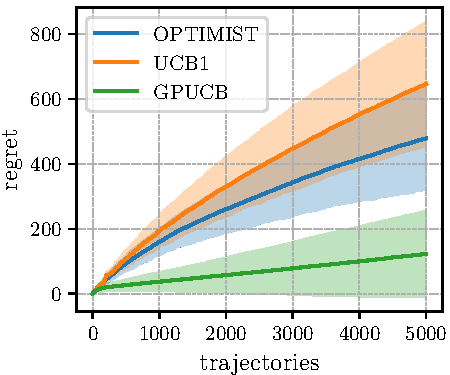
\includegraphics[width=0.3\linewidth]{plots/LQG_mu_sigma.pdf}
    \caption{Cumulative regret in the LQG experiment, comparing \algoname, UCB1 and GPUCB  when learning both the mean and the log-standard deviation parameters. (5 runs, 95\% c.i.)} 
    \label{fig:lqgVar} 
  \vskip -0.2in
\end{figure*}

%%%%%%%%%%%%%%%%%%%%%%%%%%%%%%%%%%%%%%%%%%%%%%%%%%%%%%%%%%%%%%%%%%%%%%%%%%%%%%%
%%%%%%%%%%%%%%%%%%%%%%%%%%%%%%%%%%%%%%%%%%%%%%%%%%%%%%%%%%%%%%%%%%%%%%%%%%%%%%%


\end{document}
